\documentclass[12pt]{article}
\usepackage[top=1in]{geometry}
\usepackage{graphicx}
\usepackage{amsmath}    % need for subequations
\usepackage{graphicx}   % need for figures
\usepackage{verbatim}   % useful for program listings
\usepackage{color}      % use if color is used in text
\usepackage{amsthm}
\usepackage{amsfonts}
\usepackage{amssymb}
\usepackage{subfigure}  % use for side-by-side figures
\usepackage[hidelinks]{hyperref}   % use for hypertext links, including those to external documents and URLs
\usepackage{algorithmic}
\usepackage{listings}
\usepackage[linesnumbered,ruled,vlined,commentsnumbered]{algorithm2e}
\usepackage[export]{adjustbox}
\usepackage{changepage}
\usepackage{parallel}
\usepackage{float}
\usepackage{xcolor}
\usepackage{caption}
%\usepackage{subcaption}
\usepackage{wrapfig}
\usepackage{xfrac}

\newtheorem*{conjecture}{Conjecture}
\newtheorem*{lemmastar}{Lemma}

\begin{document}

\begin{center}
 
{\bf\large The 21\textemdash or only 10\textemdash Holdout Classes Among Skelet's\\ 43 Hardly Non-Regular Turing Machines} \\
 
       %\vspace{0.5cm}
 
 
       \textbf{Daniel Briggs}
              %\vspace{0.5cm}


\end{center}

%\begin{abstract}
%\end{abstract}

\section*{Introduction}
In 2003, Skelet (Georgi Georgiev) released a 6218-line uncommented Pascal program ``bbfind'' that goes through the approximately 150 million (by the program's count) essentially distinct 5-state Turing machines and for each one attempts to either prove that it never halts when run on a blank tape or run it until it does. After a run of about two weeks, only 164 machines had stumped the program. Of these, 54 began with writing 0 to the tape, and so their runs were equivalent with an offset in number of steps to machines among the other 110. These 110 machines included 67 which were found to be ``shift recursive'' and so easily provable never to halt by hand.

Skelet dubbed the 43 remaining machines ``Hardly non-regular,'' and although his work has never been independently verified, his list has remained the starting point for anyone interested in finishing the Busy Beaver of 5 ever since.

The 27th of these 43 machines was classified as ``BL\_2'' by Skelet, and the other 42 were not classified. Note that for this reason, the machines I refer to as \#s 28\textendash43 are often referred to as 27\textendash42 by other authors\textemdash including myself, previously.

From this list of 43, \#2, \#5, and \#6 are equivalent with an offset in step number, \#13 is equivalent to \#12,  \#29 is equivalent to \#23, \#s 21, 28, and 39 are equivalent with an offset,  and \#41 is equivalent with an offset to \#30; thus we are left with 36 essentially distinct Turing machines to study.

Of these 36, \#s 16, 24, and 38 reach a phase (of at least 1 trillion steps) of equivalent action with an offset, but with several bits beyond what seems to be the working tape that are different; thus they have not been proved equivalent, but deserve to be talked about together. The situation is the same with machines \#19 \& \#42. So instead of 36 machines, we talk of 33 different studies to be made.

Of these, I (and others independently) have discovered that machines 2 (and so 5 and 6), 14, 18, and 25 are trivially proved never to halt. I also proved machines \#8, \#9, \#10, \#11, and \#12 (and so \#13) never to halt. Machines \#21 (and so \#28 and \#39), \#31 and \#32 were proved by univerz (Pavel Kropitz). univerz in fact showed the non-halting of twelve machines, but we need only reference these three for our reduction in number.

Thus there are 21 studies that need to be performed; thus this document is organized into 21 sections.
Machines \#4, 16$\sim$24$\sim$38, 19$\sim$42, 20, 23=29, 30=41, 36, 37, 40, and 43
showed that they will be of various degrees of easy but arduous in the course of producing this document,
and in fact a proof for \#36 is included herein.
\#s 34 and \#35 showed that they should be considered equivalent to each other with proof.
Of the 10 remaining classes, \#BL\_2 stands out as likely very easy, and \#15 may well be easy as well.

%\texttt{\href{https://github.com/danbriggs/Turing/blob/master/doc/record7-19-20.txt}
%{github.com/danbriggs/Turing/blob/master/doc/record7-19-20.txt}}
%is where the reader is encouraged to go to get the state diagrams for the machines.

\newpage
\tableofcontents
\clearpage
\phantomsection
\addcontentsline{toc}{section}{1}
\section*{1}

\begin{table}[H]
\begin{tabular}{lll}
86&D&$(110)^{3}(10)^{1}1i$\\
418&D&$(110)^{3}(10)^{2}(110)^{6}(10)^{1}1i$\\
1046&D&$(110)^{1}(10)^{1}(110)^{7}(10)^{2}(110)^{2}(10)^{1}(110)^{3}(10)^{1}1i$\\
3536&D&$(110)^{11}(10)^{2}(110)^{4}(10)^{1}(110)^{3}(10)^{3}(110)^{2}(10)^{1}(110)^{12}(10)^{1}1i$\\
15546&D&$(110)^{39}(10)^{2}(110)^{12}(10)^{2}(110)^{8}(10)^{1}(110)^{16}(10)^{1}(110)^{3}(10)^{1}1i$\\
54098&D&$(110)^{91}(10)^{1}(110)^{1}(10)^{1}(110)^{11}(10)^{2}(110)^{8}(10)^{1}(110)^{3}(10)^{2}(110)^{6}(10)^{1}1i$\\
79572&D&$(110)^{89}(10)^{1}(110)^{11}(10)^{1}(110)^{28}(10)^{1}(110)^{7}(10)^{2}(110)^{2}(10)^{1}(110)^{3}(10)^{1}1i$\\
2422302&D&$(110)^{139}(10)^{2}(110)^{634}(10)^{2}(110)^{76}(10)^{2}(110)^{6}(10)^{1}(110)^{11}(10)^{1}(110)^{12}(10)^{1}1i$\\
3027880&D&$(110)^{331}(10)^{2}(110)^{586}(10)^{2}(110)^{64}(10)^{3}(110)^{11}(10)^{1}(110)^{11}(10)^{1}(110)^{3}(10)^{1}1i$\\
\end{tabular}
\end{table}
The above shows steps when HNR\#1 is on the right edge of the working tape.
There are no other such steps among the first billion steps, other than nearly adjacent steps.
HNR\#1 has been perhaps the most intensely studied of all of Skelet's 43 machines over the years.
It turns out that it is certainly among the hardest nine to solve, and could well be the hardest of all.
My notes regarding HNR\#1 are scattered among old computers, dead forums, and looseleaf paper,
so it would not be appropriate to try to do the study of HNR\#1 justice here before first compiling these notes.

Although steps when it is at the right are displayed above, it is more common to study HNR\#1 using
steps when it is at the left (see figure on the following page).
Suffice it to say that it at first appears to be counting up in quaternary in its own representations
of 0, 1, 2, and 3, but it is constantly truncating the amount of working space it gives itself to count up,
and when it runs out of space to increment a number, it can end up in a variety of different ``phases.''

So new representations of what can appear on stretches of tape are defined, and replacement rules
for strings of those symbols are striven for. E.g., it leaves the left side and comes back between
the following steps:

\begin{tabular}{lll}
3284~A~$o10(110)^{10}1010(110)^{4}10(110)^{3}101010(110)^{3}1010(110)^{10}1111$\\
3822~A~$o10(110)^{8}10110100(110)^{3}10(110)^{2}11110101101001(110)^{2}10(110)^{11}1011010011,$
\end{tabular}
So one begins by letting say $X=110$ and some other alphabet assignments
and attempts to discover and prove the replacement rules among strings of them.

(HNR\#1 uses a lot of $110$ and $10$ when it is at the left as well as the right,
but for HNRs in general it is of course not the case that the same pieces will be found
when the tape head is to either side. )

This sound daunting, but it is always possible that a very general lemma that does not need to
take into account the particulars of the string can be got; in other words, ``whenever HNR\#1
has tape head at the left end of the tape and the tape is composed of such-and-such strings
in any quantity in any order, it always reaches another such configuration in the future.''
See the proof for HNR\#36 herein for comparison.

On the other hand, if its halting depends on some fine detail,
one could say that its proof is still likely quite a ways off.

\begin{figure}[H]
\centering
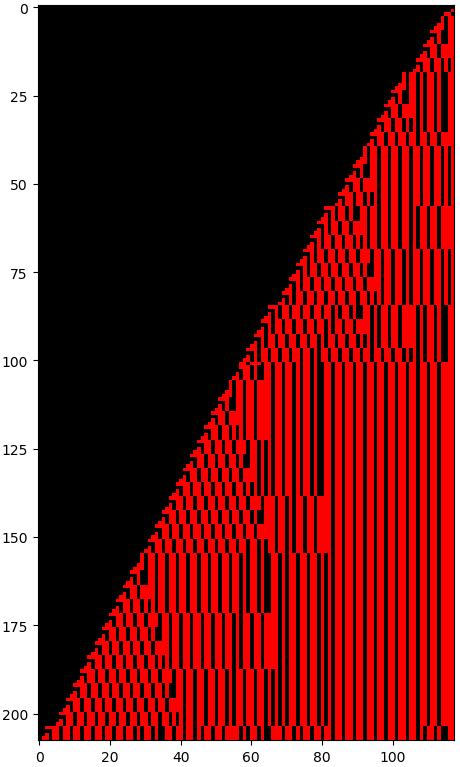
\includegraphics[width=0.8\textwidth]{1.png}
\caption{Steps through 3824 when HNR\#1 is on the left edge of the working tape.
%This and most $y$-axes in this document should be read as e.g. ``175th step where this is the case'',
%although in a few figures, the $y$-axis is labelled with the step numbers themselves.
Red means 1 and black means 0, and all such figures in this document are right-justified or left-justified,
so it should not be assumed that bits are in the exact same location from one such step to the next.}
\end{figure}

\phantomsection
\addcontentsline{toc}{section}{3}
\section*{3}
The cleanest way to study HNR\#3 is probably to inspect moments when the tape head is on the right; at these moments, the whole tape tends to be comprised of long runs of 1s with just a very few isolated 0s\textemdash often just one 0\textemdash in between. Ignoring step numbers when the tape head is on the right after it had also recently\textemdash within the past 10 steps\textemdash been at the right, we find that it achieves this configuration in state A with bit 1, state C with bit 1, state D with bit 1, or state C with bit 0\textemdash these results are for when the machine has reached the rightmost bit of the swath ever accessed, not just the current nonzero swath.

When it is in state A and there is only one 0 in between, it seems that both swaths of 1s, excluding the 1 at the tape head, may always be of even length. In order to get a handle on what it does by the time it reaches the right again afterwards, after leaving the right for at least 10 steps, I simulated runs starting from this type of configuration with two swaths of 1s of all possible even lengths up to 118, and recorded how many steps it took to get back to the right, how many swaths of 1s there were afterwards, how long the leftmost and rightmost of these were, and what state it ended up in\textemdash this time, ``on the right'' meaning at the rightmost 1. Tables \ref{tab:3nums}, \ref{tab:3swaths}, \ref{tab:3states}, \ref{tab:3lefts}, and \ref{tab:3rights} give this data for swaths of 1s of even length $\leq28$; Table \ref{tab:3steps} shows moments when the tape head is on the right when started on a blank tape.

\begin{small}
\begin{table}[H]
\begin{adjustwidth}{-1.5cm}{-1.5cm}
\texttt{
\begin{tabular}{ccccccccccccccc}
43&51&85&93&133&141&187&195&247&255&313&321&385&393&463\\
27&33&39&45&51&57&63&69&75&81&87&93&99&105&111\\
119&171&179&237&245&309&317&387&395&471&479&561&569&657&665\\
63&69&75&81&87&93&99&105&111&117&123&129&135&141&147\\
273&279&285&291&297&303&309&315&321&327&333&339&345&351&357\\
105&111&117&123&129&135&141&147&153&159&165&171&177&183&189\\
275&345&353&429&437&519&527&615&623&717&725&825&833&939&947\\
153&159&165&171&177&183&189&195&201&207&213&219&225&231&237\\
527&579&587&645&653&717&725&795&803&879&887&969&977&1065&1073\\
207&213&219&225&231&237&243&249&255&261&267&273&279&285&291\\
461&549&557&651&659&759&767&873&881&993&1001&1119&1127&1251&1259\\
267&273&279&285&291&297&303&309&315&321&327&333&339&345&351\\
849&855&861&867&873&879&885&891&897&903&909&915&921&927&933\\
333&339&345&351&357&363&369&375&381&387&393&399&405&411&417\\
677&783&791&903&911&1029&1037&1161&1169&1299&1307&1443&1451&1593&1601\\
\end{tabular}
}
\end{adjustwidth}
\caption{\label{tab:3nums}Number of steps taken to once again arrive at the rightmost 1 bit after leaving for at least 10 steps starting with configuration $1^{2m}01^{2n}i~A$ for $0\leq m,n\leq14$. Here $m$ is the row number and $n$ is the column number, both indexed from 0.}
\end{table}
\end{small}

\begin{small}
\begin{table}[H]
\texttt{
\begin{tabular}{ccccccccccccccc}
2&2&2&2&2&2&2&2&2&2&2&2&2&2&2\\
1&1&1&1&1&1&1&1&1&1&1&1&1&1&1\\
2&2&2&2&2&2&2&2&2&2&2&2&2&2&2\\
2&2&2&2&2&2&2&2&2&2&2&2&2&2&2\\
3&3&3&3&3&3&3&3&3&3&3&3&3&3&3\\
2&2&2&2&2&2&2&2&2&2&2&2&2&2&2\\
2&2&2&2&2&2&2&2&2&2&2&2&2&2&2\\
2&2&2&2&2&2&2&2&2&2&2&2&2&2&2\\
3&3&3&3&3&3&3&3&3&3&3&3&3&3&3\\
2&2&2&2&2&2&2&2&2&2&2&2&2&2&2\\
2&2&2&2&2&2&2&2&2&2&2&2&2&2&2\\
2&2&2&2&2&2&2&2&2&2&2&2&2&2&2\\
3&3&3&3&3&3&3&3&3&3&3&3&3&3&3\\
2&2&2&2&2&2&2&2&2&2&2&2&2&2&2\\
2&2&2&2&2&2&2&2&2&2&2&2&2&2&2\\
\end{tabular}}
\caption{\label{tab:3swaths}Number of swaths of 1s produced upon arriving at the rightmost 1 bit after leaving for at least 10 steps starting with configuration $1^{2m}01^{2n}i~A$ for $0\leq m,n\leq14$. Here $m$ is the row number and $n$ is the column number; both are indexed from 0. Note there seems to be no dependence on the number of 1s to the right of the 0.}
\end{table}
\end{small}

\begin{small}
\begin{table}[H]
\texttt{
\begin{tabular}{ccccccccccccccc}
A&C&A&C&A&C&A&C&A&C&A&C&A&C&A\\
D&D&D&D&D&D&D&D&D&D&D&D&D&D&D\\
C&A&C&A&C&A&C&A&C&A&C&A&C&A&C\\
D&D&D&D&D&D&D&D&D&D&D&D&D&D&D\\
D&D&D&D&D&D&D&D&D&D&D&D&D&D&D\\
D&D&D&D&D&D&D&D&D&D&D&D&D&D&D\\
C&A&C&A&C&A&C&A&C&A&C&A&C&A&C\\
D&D&D&D&D&D&D&D&D&D&D&D&D&D&D\\
C&A&C&A&C&A&C&A&C&A&C&A&C&A&C\\
D&D&D&D&D&D&D&D&D&D&D&D&D&D&D\\
C&A&C&A&C&A&C&A&C&A&C&A&C&A&C\\
D&D&D&D&D&D&D&D&D&D&D&D&D&D&D\\
D&D&D&D&D&D&D&D&D&D&D&D&D&D&D\\
D&D&D&D&D&D&D&D&D&D&D&D&D&D&D\\
C&A&C&A&C&A&C&A&C&A&C&A&C&A&C\\
\end{tabular}}
\caption{\label{tab:3states}State of the machine upon arriving at the rightmost 1 bit after leaving for at least 10 steps starting with configuration $1^{2m}01^{2n}i~A$ for $0\leq m,n\leq14$. Here $m$ is the row number and $n$ is the column number, both indexed from 0.}
\end{table}
\end{small}

\begin{small}
\begin{table}[H]
\texttt{
\begin{tabular}{ccccccccccccccc}
2&2&4&4&6&6&8&8&10&10&12&12&14&14&16\\
10&12&14&16&18&20&22&24&26&28&30&32&34&36&38\\
2&4&4&6&6&8&8&10&10&12&12&14&14&16&16\\
2&2&2&2&2&2&2&2&2&2&2&2&2&2&2\\
4&4&4&4&4&4&4&4&4&4&4&4&4&4&4\\
4&4&4&4&4&4&4&4&4&4&4&4&4&4&4\\
4&6&6&8&8&10&10&12&12&14&14&16&16&18&18\\
6&6&6&6&6&6&6&6&6&6&6&6&6&6&6\\
4&4&4&4&4&4&4&4&4&4&4&4&4&4&4\\
8&8&8&8&8&8&8&8&8&8&8&8&8&8&8\\
6&8&8&10&10&12&12&14&14&16&16&18&18&20&20\\
10&10&10&10&10&10&10&10&10&10&10&10&10&10&10\\
10&10&10&10&10&10&10&10&10&10&10&10&10&10&10\\
12&12&12&12&12&12&12&12&12&12&12&12&12&12&12\\
8&10&10&12&12&14&14&16&16&18&18&20&20&22&22\\
\end{tabular}}
\caption{\label{tab:3lefts}Length of the leftmost swath of 1s produced upon arriving at the rightmost 1 bit after leaving for at least 10 steps starting with configuration $1^{2m}01^{2n}i~A$ for $0\leq m,n\leq14$. Here $m$ is the row number and $n$ is the column number, both indexed from 0.}
\end{table}
\end{small}

\begin{small}
\begin{table}[H]
\texttt{
\begin{tabular}{ccccccccccccccc}
5&7&7&9&9&11&11&13&13&15&15&17&17&19&19\\
10&12&14&16&18&20&22&24&26&28&30&32&34&36&38\\
13&13&15&15&17&17&19&19&21&21&23&23&25&25&27\\
12&14&16&18&20&22&24&26&28&30&32&34&36&38&40\\
4&6&8&10&12&14&16&18&20&22&24&26&28&30&32\\
14&16&18&20&22&24&26&28&30&32&34&36&38&40&42\\
19&19&21&21&23&23&25&25&27&27&29&29&31&31&33\\
16&18&20&22&24&26&28&30&32&34&36&38&40&42&44\\
13&13&15&15&17&17&19&19&21&21&23&23&25&25&27\\
18&20&22&24&26&28&30&32&34&36&38&40&42&44&46\\
25&25&27&27&29&29&31&31&33&33&35&35&37&37&39\\
20&22&24&26&28&30&32&34&36&38&40&42&44&46&48\\
4&6&8&10&12&14&16&18&20&22&24&26&28&30&32\\
22&24&26&28&30&32&34&36&38&40&42&44&46&48&50\\
31&31&33&33&35&35&37&37&39&39&41&41&43&43&45\\
\end{tabular}}
\caption{\label{tab:3rights}Length of the rightmost swath of 1s produced upon arriving at the rightmost 1 bit after leaving for at least 10 steps starting with configuration $1^{2m}01^{2n}i~A$ for $0\leq m,n\leq14$. Here $m$ is the row number and $n$ is the column number, both indexed from 0.}
\end{table}
\end{small}

\begin{small}
\begin{table}[H]
\begin{Parallel}[c]{0.48\textwidth}{0.48\textwidth}
\ParallelLText{
\texttt{
\begin{tabular}{rcccl}
43&A&1&6&$1^{2}01^{4}i$\\
83&D&0&13&$1^{13}i$\\
268&A&1&18&$1^{8}01^{10}i$\\
572&D&2&30&$1^{4}01^{13}01^{13}i$\\
923&A&1&34&$1^{14}01^{20}i$\\
1137&D&1&41&$1^{6}01^{35}i$\\
1300&D&1&47&$1^{2}01^{45}i$\\
1457&D&0&53&$1^{53}i$\\
2512&A&1&58&$1^{28}01^{30}i$\\
4262&A&1&68&$1^{24}01^{44}i$\\
5244&D&2&80&$1^{10}01^{23}01^{47}i$\\
6881&C&1&84&$1^{36}01^{48}i$\\
7035&C&1&84&$1^{38}01^{46}o$\\
7731&D&1&89&$1^{18}01^{71}i$\\
8146&D&1&95&$1^{8}01^{87}i$\\
8675&D&2&106&$1^{4}01^{13}01^{89}i$\\
11762&A&1&110&$1^{52}01^{58}i$\\
16410&A&1&120&$1^{44}01^{76}i$\\
21486&C&1&130&$1^{50}01^{80}i$\\
21736&C&1&130&$1^{52}01^{78}o$\\
27456&C&1&138&$1^{52}01^{86}i$\\
27724&C&1&138&$1^{54}01^{84}o$\\
28930&D&1&143&$1^{26}01^{117}i$\\
29609&D&1&149&$1^{12}01^{137}i$\\
35900&C&1&158&$1^{72}01^{86}i$\\
36168&C&1&158&$1^{74}01^{84}o$\\
38004&D&1&163&$1^{36}01^{127}i$\\
46117&A&1&172&$1^{74}01^{98}i$\\
48005&D&1&179&$1^{36}01^{143}i$\\
57450&A&1&188&$1^{82}01^{106}i$\\
59656&D&1&195&$1^{40}01^{155}i$\\
61763&D&2&206&$1^{16}01^{33}01^{157}i$\\
71594&A&1&210&$1^{98}01^{112}i$\\
74478&D&1&217&$1^{48}01^{169}i$\\
86025&C&2&231&$1^{10}01^{109}01^{112}i$\\
86371&C&2&231&$1^{10}01^{111}01^{110}o$\\
99063&A&1&234&$1^{68}01^{166}i$\\
\end{tabular}}}
\ParallelRText{
\texttt{
\begin{tabular}{rcccl}
114997&A&1&244&$1^{102}01^{142}i$\\
118151&D&1&251&$1^{50}01^{201}i$\\
119604&D&1&257&$1^{24}01^{233}i$\\
121147&D&2&268&$1^{10}01^{23}01^{235}i$\\
137166&C&1&272&$1^{130}01^{142}i$\\
137602&C&1&272&$1^{132}01^{140}o$\\
159556&A&1&280&$1^{104}01^{176}i$\\
167144&D&2&292&$1^{40}01^{73}01^{179}i$\\
184393&C&1&296&$1^{132}01^{164}i$\\
184895&C&1&296&$1^{134}01^{162}o$\\
189755&D&1&301&$1^{66}01^{235}i$\\
191778&D&1&307&$1^{32}01^{275}i$\\
193873&D&3&323&$1^{4}01^{23}01^{19}01^{277}i$\\
214312&A&2&327&$1^{4}01^{165}01^{158}i$\\
240390&C&1&332&$1^{86}01^{246}i$\\
241138&C&1&332&$1^{88}01^{244}o$\\
247234&D&2&342&$1^{34}01^{63}01^{245}i$\\
272173&A&1&346&$1^{160}01^{186}i$\\
286901&D&3&363&$1^{16}01^{75}01^{83}01^{189}i$\\
307178&A&2&367&$1^{16}01^{173}01^{178}i$\\
338230&C&1&372&$1^{108}01^{264}i$\\
339032&C&1&372&$1^{110}01^{262}o$\\
342914&D&1&377&$1^{54}01^{323}i$\\
344841&D&1&383&$1^{26}01^{357}i$\\
346240&D&1&389&$1^{12}01^{377}i$\\
380071&C&1&398&$1^{192}01^{206}i$\\
380699&C&1&398&$1^{194}01^{204}o$\\
389825&D&1&403&$1^{96}01^{307}i$\\
396816&D&3&419&$1^{10}01^{49}01^{51}01^{309}i$\\
429039&A&2&423&$1^{10}01^{207}01^{206}i$\\
471335&C&1&428&$1^{116}01^{312}i$\\
472281&C&1&428&$1^{118}01^{310}o$\\
476709&D&1&433&$1^{58}01^{375}i$\\
478906&D&1&439&$1^{28}01^{411}i$\\
522833&A&1&448&$1^{214}01^{234}i$\\
533739&D&1&455&$1^{106}01^{349}i$\\
537694&D&1&461&$1^{52}01^{409}i$\\
\end{tabular}}}
\end{Parallel}
\caption{\label{tab:3steps}The step numbers when the tape head was at the rightmost bit of the swath ever accessed after leaving the right for at least 10 steps; what state the machine was in; how many intermediate zeros there were; how many 1s there were other than at the tape head; what the tape looked like. Run started on a blank tape.}
\end{table}
\end{small}

\clearpage
Repeating the analysis done in Tables \ref{tab:3nums}, \ref{tab:3swaths}, \ref{tab:3states}, \ref{tab:3lefts}, and \ref{tab:3rights}, but with the machine starting in state C instead of A gives much simpler data: there are always two swaths; the number of steps and lengths of the left and right swaths are linear functions of the lengths of the original swaths; the machine ends up in state D as long as the right swath has at least six 1s. The machine starting in state D is exactly analogous to starting in state A, but the tape head is one bit further to the right and the step number is advanced by three. C with tape head at a 0 bit always comes from D with tape head at a 1 bit but otherwise of the same form.

Thus, it would suffice to understand the patterns shown in Tables \ref{tab:3nums}, \ref{tab:3swaths}, \ref{tab:3states}, \ref{tab:3lefts}, and \ref{tab:3rights} to predict the action of HNR\#3 from situations consisting of at most two swaths of 1s. However, situations with more than two swaths as shown in Table \ref{tab:3steps} may have to be understood separately, and could increase the difficulty of showing that HNR\#3 never halts or accelerating it until it does.

Out of the first billion steps, the maximum number of swaths of 1s when the tape head is on the right is 6, and this first occurs at step 6333029, when the machine is in state D, and the tape is \texttt{$1^4~0~1^{23}~0~1^{53}~0~1^{197}~0~1^{259}~0~1^{550}$}.

The table also shows quite a few pairs of steps where the first of two 1's exponents
is halved and one subtracted; the criteria under which this does or does not occur
are not clear. For this reason, HNR\#3 could easily prove to be as difficult as
say the Collatz conjecture.

An argument backtracking from a halt state may be capable of sidestepping all this detailed analysis,
but this has so far proven not to be the case with any of the HNRs (although see HNR\#36 where halting
would be achieved iff an even number of 0s appeared between the tape head and the first 1 in state D
while it always has an odd number of 0s in that position.).
%\begin{table}[H]
%\texttt{\begin{tabular}{rccccc}
%&A&B&C&D&E\\
%0&C1L&H1L&D1R&A1R&C0L\\
%1&A0R&E1L&B0L&C1R&D1L
%\end{tabular}}
%\label{tab:HNR3}
%\end{table}
%\noindent that 01o A and 01o E are the only ways to achieve halting; these must come from 0o0 D, 010i B, respectively; the former is a dead-end, whereas the latter comes from 0101i C; unfortunately, this branches into three possibilities: 01011o A, 010o1 D, and 01011o E. These respectively come from 0101o0 D, 0100i E, and 010110i B; these, from 010i00 C, 01001i B, and 0101101i C;



\clearpage
\phantomsection
\addcontentsline{toc}{section}{4}
\section*{4}

Machine 4 seems to be a trivial one, the proof just needs to be carried out. It counts up in binary using 11 as 0 and 10 as 1, with less significant digits to the left, on the left side of the tape, with an additional o11 at the left end in C.
Then after a number of steps increasing by a constant difference of 12 modified by four times the location in the number of the 0 to be turned into a 1 (increasing when that bit is \emph{closer}), it produces the next number, written in the same binary scheme,
with an extra number 0 (again, written 11) as padding on the right before the ending 011. For example,

\begin{small}
\begin{table}[H]
\texttt{
\begin{tabular}{rclcl}
882&  C&           o1110101110111111111111111011& 11.& Then after 145,\\
1027& C&         o111111101011111111111111111011& 12.& Then after 165 (+20 3/1),\\
1192& C&       o11101110101111111111111111111011& 13.& Then after 173 (+8 1/2),\\
1365& C&     o1111101010111111111111111111111011& 14.& Then after 189 (+16 2/1),\\
1554& C&   o111010101011111111111111111111111011& 15.& Then after 185 (-4 1/5),\\
1739& C& o11111111111011111111111111111111111011& 16.& Then after 213 (+28).
\end{tabular}}
\caption{\label{tab:4}Machine 4. The numbers before and after the slash portray which bit in is to be turned from a 0 to a 1 previously/currently. The difference between the two numbers determines the multiple of 4 offset from 12 more the step difference will be above the previous step difference.}
\end{table}
\end{small}

Thus, as it is creating more space for itself to count up in far faster than it is counting up, it will never halt.

%\clearpage adds a blank page. Next table too large?
\phantomsection
\addcontentsline{toc}{section}{7}
\section*{7}

\begin{small}
\begin{table}[H]
\begin{Parallel}[c]{0.48\textwidth}{0.48\textwidth}
\ParallelLText{
\texttt{
\begin{tabular}{rcr}
33&A&$1^{2}0^{1}1^{2}$\\
57&C&$1^{10}$\\
188&D&$1^{9}0^{1}1^{6}$\\
276&C&$1^{20}0^{1}1^{2}$\\
355&C&$1^{28}$\\
746&A&$1^{19}0^{1}1^{14}$\\
810&A&$1^{16}0^{1}1^{16}$\\
1602&D&$1^{19}0^{1}1^{23}0^{1}1^{4}$\\
2234&A&$1^{35}0^{1}1^{16}$\\
2346&A&$1^{32}0^{1}1^{18}$\\
2640&C&$1^{48}0^{1}1^{8}$\\
3049&C&$1^{50}0^{1}1^{13}0^{1}1^{4}$\\
4426&D&$1^{39}0^{1}1^{32}$\\
5816&C&$1^{42}0^{1}1^{19}0^{1}1^{23}0^{1}1^{4}$\\
7139&D&$1^{41}0^{1}1^{47}0^{1}1^{4}$\\
9473&D&$1^{69}0^{1}1^{28}$\\
12905&A&$1^{65}0^{1}1^{42}$\\
13107&A&$1^{62}0^{1}1^{44}$\\
17183&A&$1^{73}0^{1}1^{42}$\\
17409&A&$1^{70}0^{1}1^{44}$\\
21971&A&$1^{77}0^{1}1^{46}$\\
22209&A&$1^{74}0^{1}1^{48}$\\
26915&A&$1^{65}0^{1}1^{61}0^{1}1^{10}$\\
27117&A&$1^{62}0^{1}1^{63}0^{1}1^{10}$\\
31493&D&$1^{95}0^{1}1^{44}$\\
37941&D&$1^{89}0^{1}1^{60}$\\
45261&A&$1^{99}0^{1}1^{60}$\\
45565&A&$1^{96}0^{1}1^{62}$\\
47041&C&$1^{134}0^{1}1^{30}$\\
47840&C&$1^{156}0^{1}1^{14}$\\
48453&C&$1^{170}0^{1}1^{6}$\\
49018&C&$1^{180}0^{1}1^{2}$\\
49577&C&$1^{188}$\\
57768&A&$1^{99}0^{1}1^{94}$\\
58072&A&$1^{96}0^{1}1^{96}$\\
64426&C&$1^{98}0^{1}1^{51}0^{1}1^{49}0^{1}1^{10}$\\
70891&D&$1^{101}0^{1}1^{101}0^{1}1^{10}$\\
81739&D&$1^{153}0^{1}1^{64}$\\
93763&A&$1^{113}0^{1}1^{97}0^{1}1^{23}0^{1}1^{4}$\\
94109&A&$1^{110}0^{1}1^{99}0^{1}1^{23}0^{1}1^{4}$\\
\end{tabular}}}
\ParallelRText{
\texttt{
\begin{tabular}{rcr}
105757&D&$1^{155}0^{1}1^{81}0^{1}1^{4}$\\
120999&A&$1^{161}0^{1}1^{84}$\\
121489&A&$1^{158}0^{1}1^{86}$\\
123997&C&$1^{208}0^{1}1^{42}$\\
125270&C&$1^{236}0^{1}1^{20}$\\
141651&D&$1^{141}0^{1}1^{124}$\\
162381&A&$1^{173}0^{1}1^{102}$\\
162907&A&$1^{170}0^{1}1^{104}$\\
170467&C&$1^{172}0^{1}1^{73}0^{1}1^{40}$\\
186702&A&$1^{161}0^{1}1^{128}$\\
187192&A&$1^{158}0^{1}1^{130}$\\
191812&C&$1^{230}0^{1}1^{64}$\\
211699&A&$1^{151}0^{1}1^{135}0^{1}1^{23}0^{1}1^{4}$\\
212159&A&$1^{148}0^{1}1^{137}0^{1}1^{23}0^{1}1^{4}$\\
232791&A&$1^{213}0^{1}1^{99}0^{1}1^{4}$\\
233437&A&$1^{210}0^{1}1^{101}0^{1}1^{4}$\\
259509&D&$1^{207}0^{1}1^{112}$\\
284371&D&$1^{163}0^{1}1^{149}0^{1}1^{22}$\\
309195&A&$1^{233}0^{1}1^{106}$\\
309901&A&$1^{230}0^{1}1^{108}$\\
340719&A&$1^{205}0^{1}1^{142}$\\
341341&A&$1^{202}0^{1}1^{144}$\\
370731&A&$1^{177}0^{1}1^{155}0^{1}1^{28}$\\
371269&A&$1^{174}0^{1}1^{157}0^{1}1^{28}$\\
399339&D&$1^{245}0^{1}1^{118}$\\
403579&C&$1^{312}0^{1}1^{58}$\\
405584&C&$1^{348}0^{1}1^{28}$\\
438615&D&$1^{203}0^{1}1^{182}$\\
446809&C&$1^{302}0^{1}1^{90}$\\
449912&C&$1^{354}0^{1}1^{44}$\\
487277&A&$1^{219}0^{1}1^{188}$\\
487941&A&$1^{216}0^{1}1^{190}$\\
496785&C&$1^{318}0^{1}1^{94}$\\
500104&C&$1^{372}0^{1}1^{46}$\\
501965&C&$1^{402}0^{1}1^{22}$\\
503430&C&$1^{420}0^{1}1^{10}$\\
504787&C&$1^{432}0^{1}1^{4}$\\
546044&D&$1^{227}0^{1}1^{218}$\\
557280&C&$1^{344}0^{1}1^{108}$\\
608971&D&$1^{261}0^{1}1^{200}$\\
\end{tabular}}}
\end{Parallel}
\caption{\label{tab:7}HNR\#7, tapehead at leftmost bit. See similarities of HNR\#3.}
\end{table}
\end{small}

\clearpage
\phantomsection
\addcontentsline{toc}{section}{15}
\section*{15}

\begin{tiny}
\begin{table}[H]
\texttt{
\hspace*{-1.55in}
\setlength\tabcolsep{2pt}
\begin{tabular}{rrrrr}
31167&C&$i1^{0}0111111101011111110101011111010111010101011101111111010101010101011$&diff&off\\
31203&C&$i1^{4}01110101{\textcolor{red}{1}}1011111110101011111010111010101011101111111010101010101011$&+36&0\\
31267&C&$i1^{8}011101{\textcolor{red}{1}}111011111110101011111010111010101011101111111010101010101011$&+64&-8\\
31407&C&$i1^{12}0111011101{\textcolor{red}{1}}11111110101011111010111010101011101111111010101010101011$&+140&-4\\
31703&C&$i1^{16}011101110101010101{\textcolor{red}{1}}101011111010111010101011101111111010101010101011$&+296&8\\
32271&C&$i1^{20}011101110101{\textcolor{red}{1}}101011101011111010111010101011101111111010101010101011$&+568&-8\\
33415&C&$i1^{24}01110111010111{\textcolor{red}{1}}1011101011111010111010101011101111111010101010101011$&+1144&-8\\
35711&C&$i1^{28}0111011101011111{\textcolor{red}{1}}11101011111010111010101011101111111010101010101011$&+2296&-8\\
40315&C&$i1^{32}01110111010111111101{\textcolor{red}{1}}1011111010111010101011101111111010101010101011$&+4604&-4\\
49527&C&$i1^{36}0111011101011111110101{\textcolor{red}{1}}11111010111010101011101111111010101010101011$&+9212&-4\\
67963&C&$i1^{40}0111011101011111110101010101{\textcolor{red}{1}}10111010101011101111111010101010101011$&+18436&4\\
104819&C&$i1^{44}011101110101111111010101{\textcolor{red}{1}}101110111010101011101111111010101010101011$&+36856&-8\\
178539&C&$i1^{48}01110111010111111101010111{\textcolor{red}{1}}1110111010101011101111111010101010101011$&+73720&-8\\
325991&C&$i1^{52}011101110101111111010101111101{\textcolor{red}{1}}111010101011101111111010101010101011$&+147452&-4\\
620903&C&$i1^{56}0111011101011111110101011111010101{\textcolor{red}{1}}10101011101111111010101010101011$&+294912&0\\
1210719&C&$i1^{60}01110111010111111101010111110101{\textcolor{red}{1}}1110101011101111111010101010101011$&+589816&-8\\
2390363&C&$i1^{64}011101110101111111010101111101011101{\textcolor{red}{1}}101011101111111010101010101011$&+1179644&-4\\
4749655&C&$i1^{68}01110111010111111101010111110101110101{\textcolor{red}{1}}1011101111111010101010101011$&+2359292&-4\\
9468243&C&$i1^{72}0111011101011111110101011111010111010101{\textcolor{red}{1}}11101111111010101010101011$&+4718588&-4\\
18905427&C&$i1^{76}01110111010111111101010111110101110101010101{\textcolor{red}{1}}1111111010101010101011$&+9437184&0\\
37779787&C&$i1^{80}011101110101111111010101111101011101010101{\textcolor{red}{1}}111111111010101010101011$&+18874360&-8\\
75528531&C&$i1^{84}0111011101011111110101011111010111010101011101010101{\textcolor{red}{1}}10101010101011$&+37748744&8\\
151025995&C&$i1^{88}0111011101011111110101011111010111010101011101{\textcolor{red}{1}}10101110101010101011$&+75497464&-8\\
302020931&C&$i1^{92}011101110101111111010101111101011101010101110111{\textcolor{red}{1}}101110101010101011$&+150994936&-8\\
604010811&C&$i1^{96}01110111010111111101010111110101110101010111011111{\textcolor{red}{1}}1110101010101011$&+301989880&-8\\
1207990583&C&$i1^{100}011101110101111111010101111101011101010101110111111101{\textcolor{red}{1}}101010101011$&+603979772&-4\\
2415950131&C&$i1^{104}01110111010111111101010111110101110101010111011111110101{\textcolor{red}{1}}1010101011$&+1207959548&-4\\
4831869231&C&$i1^{108}0111011101011111110101011111010111010101011101111111010101{\textcolor{red}{1}}10101011$&+2415919100&-4\\
38654736675&C&$i1^{120}0111011101011111110101011111010111010101011101111111010101010101{\textcolor{red}{1}}11$&+19327352828&-4\\
\end{tabular}}
\caption{\label{tab:15}Machine 15. Let $i$ be the row in the table above, indexed from $-1$; let $x_i=36*2^{i}.$ Let $d_i$ be the
difference in step number between the $i$th row and the $i-1$st row, and let $k_i$ be the place of the first $1$ bit that was a
$0$ bit in the previous line, indexing from 0 just after the compressed portion. It is observed that $d_i-x_i$ relates to $k_i-2i$
in the following linear fashion: $d_i-x_i=-16+2(k_i-2i).$ Also, $k_i-2i$ always seems to be 2, 4, 6, 8, or 10. Also, the positions of the new
1s, highlighted in red, seem to be injective and surjective among every other position throughout the swath other than at the very end.
Furthermore, once all this work is done, only the second 0 and the last 0 have been changed, and everything else in its ``workspace''
is as at the beginning.}
\end{table}
\end{tiny}

\newpage

\begin{table}[H]
\texttt{
\hspace*{-1.55in}
\setlength\tabcolsep{2pt}
\begin{tiny}
\begin{tabular}{rrrrr}
76761382320&C&$i1^{0}011111111111111111111111111101010101010111111111010111010101010111011111010111010101111101110101110101010101111101110111110111110111(01)^{30}1$&diff&off\\
76761382396&C&$i1^{4}0111010101010101010101010101{\textcolor{red}{1}}1010101010111111111010111010101010111011111010111010101111101110101110101010101111101110111110111110111(01)^{30}1$&+76&40\\
76761382460&C&$i1^{8}011101{\textcolor{red}{1}}10101010101010101010111010101010111111111010111010101010111011111010111010101111101110101110101010101111101110111110111110111(01)^{30}1$&+64&-8\\
76761382596&C&$i1^{12}01110111{\textcolor{red}{1}}101010101010101010111010101010111111111010111010101010111011111010111010101111101110101110101010101111101110111110111110111(01)^{30}1$&+136&-8\\
76761382876&C&$i1^{16}0111011111{\textcolor{red}{1}}1010101010101010111010101010111111111010111010101010111011111010111010101111101110101110101010101111101110111110111110111(01)^{30}1$&+280&-8\\
76761383444&C&$i1^{20}011101111111{\textcolor{red}{1}}10101010101010111010101010111111111010111010101010111011111010111010101111101110101110101010101111101110111110111110111(01)^{30}1$&+568&-8\\
76761384588&C&$i1^{24}01110111111111{\textcolor{red}{1}}101010101010111010101010111111111010111010101010111011111010111010101111101110101110101010101111101110111110111110111(01)^{30}1$&+1144&-8\\
76761386884&C&$i1^{28}0111011111111111{\textcolor{red}{1}}1010101010111010101010111111111010111010101010111011111010111010101111101110101110101010101111101110111110111110111(01)^{30}1$&+2296&-8\\
76761391484&C&$i1^{32}011101111111111111{\textcolor{red}{1}}10101010111010101010111111111010111010101010111011111010111010101111101110101110101010101111101110111110111110111(01)^{30}1$&+4600&-8\\
76761400692&C&$i1^{36}01110111111111111111{\textcolor{red}{1}}101010111010101010111111111010111010101010111011111010111010101111101110101110101010101111101110111110111110111(01)^{30}1$&+9208&-8\\
76761419116&C&$i1^{40}0111011111111111111111{\textcolor{red}{1}}1010111010101010111111111010111010101010111011111010111010101111101110101110101010101111101110111110111110111(01)^{30}1$&+18424&-8\\
76761455972&C&$i1^{44}011101111111111111111111{\textcolor{red}{1}}10111010101010111111111010111010101010111011111010111010101111101110101110101010101111101110111110111110111(01)^{30}1$&+36856&-8\\
76761529692&C&$i1^{48}01110111111111111111111111{\textcolor{red}{1}}111010101010111111111010111010101010111011111010111010101111101110101110101010101111101110111110111110111(01)^{30}1$&+73720&-8\\
76761677144&C&$i1^{52}011101111111111111111111111101{\textcolor{red}{1}}10101010111111111010111010101010111011111010111010101111101110101110101010101111101110111110111110111(01)^{30}1$&+147452&-4\\
76761972052&C&$i1^{56}01110111111111111111111111110101{\textcolor{red}{1}}101010111111111010111010101010111011111010111010101111101110101110101010101111101110111110111110111(01)^{30}1$&+294908&-4\\
76762561872&C&$i1^{60}0111011111111111111111111111010101{\textcolor{red}{1}}1010111111111010111010101010111011111010111010101111101110101110101010101111101110111110111110111(01)^{30}1$&+589820&-4\\
76763741516&C&$i1^{64}011101111111111111111111111101010101{\textcolor{red}{1}}10111111111010111010101010111011111010111010101111101110101110101010101111101110111110111110111(01)^{30}1$&+1179644&-4\\
76766100808&C&$i1^{68}01110111111111111111111111110101010101{\textcolor{red}{1}}111111111010111010101010111011111010111010101111101110101110101010101111101110111110111110111(01)^{30}1$&+2359292&-4\\
76770819412&C&$i1^{72}011101111111111111111111111101010101010101010101{\textcolor{red}{1}}10111010101010111011111010111010101111101110101110101010101111101110111110111110111(01)^{30}1$&+4718604&12\\
76780256588&C&$i1^{76}0111011111111111111111111111010101010101{\textcolor{red}{1}}1010101110111010101010111011111010111010101111101110101110101010101111101110111110111110111(01)^{30}1$&+9437176&-8\\
76799130948&C&$i1^{80}011101111111111111111111111101010101010111{\textcolor{red}{1}}10101110111010101010111011111010111010101111101110101110101010101111101110111110111110111(01)^{30}1$&+18874360&-8\\
76836879676&C&$i1^{84}01110111111111111111111111110101010101011111{\textcolor{red}{1}}101110111010101010111011111010111010101111101110101110101010101111101110111110111110111(01)^{30}1$&+37748728&-8\\
76912377140&C&$i1^{88}0111011111111111111111111111010101010101111111{\textcolor{red}{1}}1110111010101010111011111010111010101111101110101110101010101111101110111110111110111(01)^{30}1$&+75497464&-8\\
77063372080&C&$i1^{92}01110111111111111111111111110101010101011111111101{\textcolor{red}{1}}111010101010111011111010111010101111101110101110101010101111101110111110111110111(01)^{30}1$&+150994940&-4\\
77365361968&C&$i1^{96}011101111111111111111111111101010101010111111111010101{\textcolor{red}{1}}10101010111011111010111010101111101110101110101010101111101110111110111110111(01)^{30}1$&+301989888&0\\
77969341736&C&$i1^{100}0111011111111111111111111111010101010101111111110101{\textcolor{red}{1}}1110101010111011111010111010101111101110101110101010101111101110111110111110111(01)^{30}1$&+603979768&-8\\
79177301284&C&$i1^{104}01110111111111111111111111110101010101011111111101011101{\textcolor{red}{1}}101010111011111010111010101111101110101110101010101111101110111110111110111(01)^{30}1$&+1207959548&-4\\
\end{tabular}
\end{tiny}}
\caption{\label{tab:15-2}The machine's behavior after returning to the left at step 76761382305 B. It has set up a new task for itself
in that it has written new stuff further to the right of where it had stuff previously, and it has gone back to having no 1s to the left
of the workspace. It repeats its prior behavior, again taking nearly exactly $36*2^{n/4}$ steps to install a new 1 and return to the left,
where $n$ is the number of 1s after the $i$ on the left (the first difference is significantly greater than $36$ since the first new 1 to install is so far to the right),
again injectively and bijectively ostensibly until $n/4$ is at or near $93,$ and then when $n=94$ it would likely either write a new workspace for itself
or do something new entirely. So in order to continue analyzing this machine effectively, an acceleration should be written that is able to
automate away these $36*2^{93}$ or so steps. After all this work is done, seemingly only the second 0 and the last 0 would be altered,
all the rest of the bits in the workspace becoming as they were before the work started.}
\end{table}

Ostensibly the pack of 1s on the left is telling the machine to go to at least the $\frac n4+2$nd even bit after the pack
(indexing from 0 at the first bit after the pack) and turn the first 0 bit encountered from that point on into a 1,
turning alternate 1 bits that it encounters between that index and that bit back into 0s. The most primitive way that
a Turing machine could carry out a task like this of course takes exponential time in the number of 1 bits on the left,
matching the pattern in step differences that we see, and this would also explain why the bits of the working tape end up
nearly exactly as they were before the work began once the machine has accomplished this for each bit. 

\newpage

\begin{conjecture}
For any string $x=a_0\ldots a_m$
with each of the $a_j$ being $10$ or $11,$
and any nonnegative integer $n\leq m,$
let $j$ be the least index $j\geq n$ such that $a_j=10$;
suppose such index exists.
Then
$$0^4 i1^{4n}011x~\texttt{C}~\vdash~
i1^{4n+4}011\overline x~\texttt{C}\quad\quad36\cdot2^n-8+4(j-n),$$
where $\overline x = 
a_0a_1\ldots a_{n-1}\overline{a_{n}}\hspace{.08883em}\overline{a_{n+1}}\ldots\overline{a_j}
a_{j+1}\ldots a_m,$ for $a=10,$ $\overline a=11,$ and vice versa.
\end{conjecture}

The conjecture has been verified to produce each subsequent line of either of the two tables above
from any given current line running the Python script found at 
\href{https://github.com/danbriggs/Turing/blob/master/paper/accelerate\_15\_old.py}
{github.com/danbriggs/Turing/blob/master/paper/accelerate\_15\_old.py},
which uses
\href{https://github.com/danbriggs/Turing/blob/master/paper/stepfiguration.py}{stepfiguration.py}
from the same directory. Assuming the conjecture is true,
one obtains
\begin{align*}
&356526731314189519247709158424~\texttt{C}\\
&i1^{372}0111011111111111111111111111010101010101111111110101110101010101110/\\
&11111010111010101111101110101110101010101111101110111110111110111010101/\\
&0101010101010101010101010101010101010101010101010101111/\\
\end{align*}
i.e., the machine runs for at least 356 octillion or $3.56\cdot10^{29}$ steps.

Pushing beyond this 356 octillion boundary will require applying the specific lemmas that would
combine to provide the conjecture above in a manner very similar to that that would prove the conjecture.
Scratch notes can be found at
\href{https://github.com/danbriggs/Turing/blob/master/paper/noteson15.txt}{noteson15.txt}.

\clearpage
\phantomsection
\addcontentsline{toc}{section}{16$\sim$24$\sim$38}
\section*{16$\sim$24$\sim$38}

\begin{figure}[H]
\centering
\begin{subfigure}
\centering
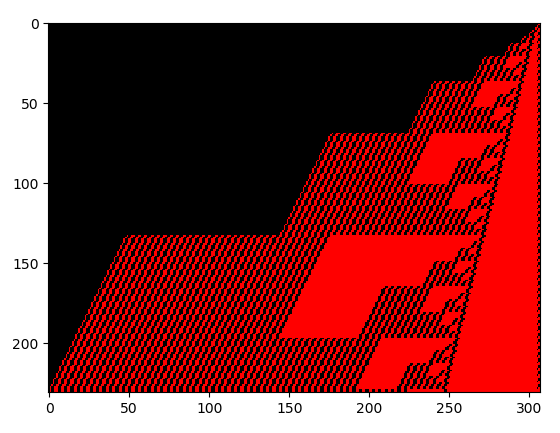
\includegraphics[width=0.45\textwidth]{16.png}
\label{fig:16}
\end{subfigure}
\hfill
\begin{subfigure}
\centering
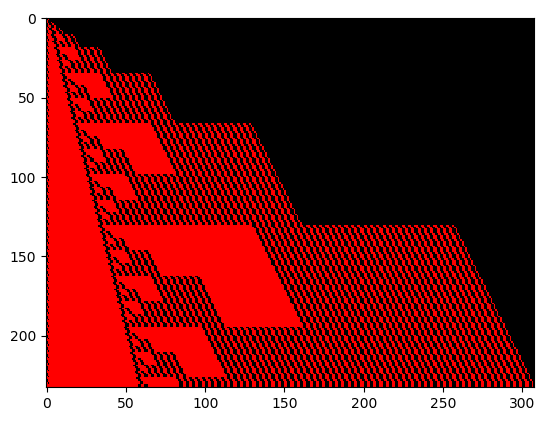
\includegraphics[width=0.45\textwidth]{24.png}
\label{fig:24}
\end{subfigure}
\caption{HNRs \#16 \& 24, tape head at extreme for up to 30000 steps.}
\end{figure}

\begin{figure}[H]
\centering
\begin{subfigure}
\centering
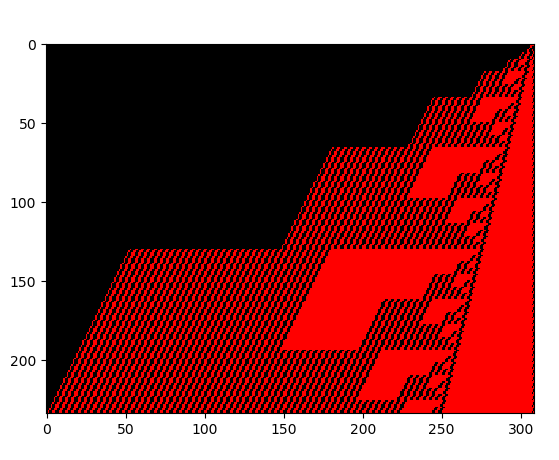
\includegraphics[width=0.45\textwidth]{38-r.png}
\label{fig:38r}
\end{subfigure}
\hfill
\begin{subfigure}
\centering
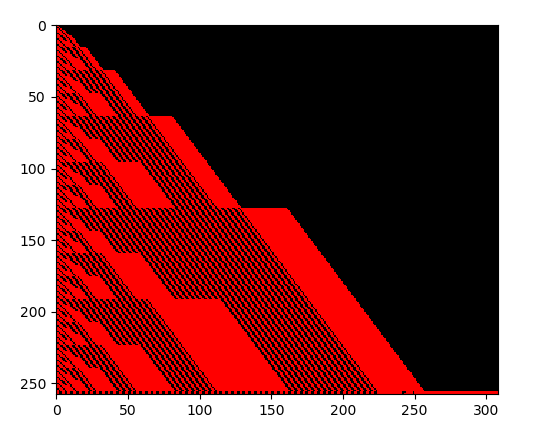
\includegraphics[width=0.45\textwidth]{38.png}
\label{fig:38l}
\end{subfigure}
\caption{HNR \#38, head at right, left resp. These three machines require but a routine proof.}
\end{figure}




\clearpage
\phantomsection
\addcontentsline{toc}{section}{17}
\section*{17}



\begin{table}[H]
\begin{Parallel}[c]{0.48\textwidth}{0.48\textwidth}
\ParallelLText{
\texttt{
\begin{scriptsize}
\begin{tabular}{rrl}
0&A&$o$\\
2&C&$i$\\
18&B&$(10)^{1}1i$\\
34&C&$(10)^{2}i$\\
66&B&$(10)^{1}1(10)^{1}1i$\\
88&D&$(10)^{2}1(10)^{1}i$\\
89&B&$(10)^{2}1(10)^{1}1o$\\
90&C&$(10)^{2}1(10)^{2}o$\\
91&D&$(10)^{2}1(10)^{2}0o$\\
95&C&$(10)^{2}1(10)^{2}1i$\\
219&C&$(10)^{4}1(10)^{2}1i$\\
335&B&$(10)^{4}1(10)^{2}1(10)^{1}1i$\\
451&C&$(10)^{4}1(10)^{2}1(10)^{2}i$\\
583&B&$(10)^{4}1(10)^{4}1(10)^{1}1i$\\
723&C&$(10)^{6}1(10)^{2}1(10)^{2}i$\\
895&B&$(10)^{1}1(10)^{4}1(10)^{4}1(10)^{1}1i$\\
1111&C&$(10)^{8}1(10)^{2}1(10)^{2}i$\\
1323&B&$(10)^{3}1(10)^{4}1(10)^{4}1(10)^{1}1i$\\
1675&C&$(10)^{8}1(10)^{4}1(10)^{2}i$\\
1911&B&$(10)^{3}1(10)^{6}1(10)^{4}1(10)^{1}1i$\\
2335&C&$(10)^{1}1(10)^{8}1(10)^{4}1(10)^{2}i$\\
2679&B&$(10)^{3}1(10)^{8}1(10)^{4}1(10)^{1}1i$\\
3175&C&$(10)^{3}1(10)^{8}1(10)^{4}1(10)^{2}i$\\
3687&B&$(10)^{3}1(10)^{8}1(10)^{6}1(10)^{1}1i$\\
4223&C&$(10)^{3}1(10)^{10}1(10)^{4}1(10)^{2}i$\\
4807&B&$(10)^{5}1(10)^{8}1(10)^{6}1(10)^{1}1i$\\
5507&C&$(10)^{3}1(10)^{12}1(10)^{4}1(10)^{2}i$\\
6163&B&$(10)^{7}1(10)^{8}1(10)^{6}1(10)^{1}1i$\\
6545&D&$(10)^{12}1(10)^{8}1(10)^{2}1(10)^{1}i$\\
6546&B&$(10)^{12}1(10)^{8}1(10)^{2}1(10)^{1}1o$\\
6547&C&$(10)^{12}1(10)^{8}1(10)^{2}1(10)^{2}o$\\
6548&D&$(10)^{12}1(10)^{8}1(10)^{2}1(10)^{2}0o$\\
6552&C&$(10)^{12}1(10)^{8}1(10)^{2}1(10)^{2}1i$\\
8200&C&$(10)^{12}1(10)^{8}1(10)^{4}1(10)^{2}1i$\\
9944&C&$(10)^{14}1(10)^{8}1(10)^{4}1(10)^{2}1i$\\
11988&C&$(10)^{16}1(10)^{8}1(10)^{4}1(10)^{2}1i$\\
13212&B&$(10)^{16}1(10)^{8}1(10)^{4}1(10)^{2}1(10)^{1}1i$\\
14436&C&$(10)^{16}1(10)^{8}1(10)^{4}1(10)^{2}1(10)^{2}i$\\
15676&B&$(10)^{16}1(10)^{8}1(10)^{4}1(10)^{4}1(10)^{1}1i$\\
16924&C&$(10)^{16}1(10)^{8}1(10)^{6}1(10)^{2}1(10)^{2}i$\\
18204&B&$(10)^{16}1(10)^{10}1(10)^{4}1(10)^{4}1(10)^{1}1i$\\
19524&C&$(10)^{18}1(10)^{8}1(10)^{6}1(10)^{2}1(10)^{2}i$\\
20940&B&$(10)^{1}1(10)^{16}1(10)^{10}1(10)^{4}1(10)^{4}1(10)^{1}1i$\\
22480&C&$(10)^{20}1(10)^{8}1(10)^{6}1(10)^{2}1(10)^{2}i$\\
\end{tabular}
\end{scriptsize}}}
\ParallelRText{
\texttt{
\begin{scriptsize}
\begin{tabular}{rrl}
24032&B&$(10)^{3}1(10)^{16}1(10)^{10}1(10)^{4}1(10)^{4}1(10)^{1}1i$\\
25876&C&$(10)^{20}1(10)^{10}1(10)^{6}1(10)^{2}1(10)^{2}i$\\
27500&B&$(10)^{3}1(10)^{18}1(10)^{10}1(10)^{4}1(10)^{4}1(10)^{1}1i$\\
29512&C&$(10)^{1}1(10)^{20}1(10)^{10}1(10)^{6}1(10)^{2}1(10)^{2}i$\\
31388&B&$(10)^{3}1(10)^{20}1(10)^{10}1(10)^{4}1(10)^{4}1(10)^{1}1i$\\
33568&C&$(10)^{3}1(10)^{20}1(10)^{10}1(10)^{6}1(10)^{2}1(10)^{2}i$\\
35780&B&$(10)^{3}1(10)^{20}1(10)^{12}1(10)^{4}1(10)^{4}1(10)^{1}1i$\\
38048&C&$(10)^{3}1(10)^{22}1(10)^{10}1(10)^{6}1(10)^{2}1(10)^{2}i$\\
40428&B&$(10)^{5}1(10)^{20}1(10)^{12}1(10)^{4}1(10)^{4}1(10)^{1}1i$\\
43004&C&$(10)^{3}1(10)^{24}1(10)^{10}1(10)^{6}1(10)^{2}1(10)^{2}i$\\
45552&B&$(10)^{7}1(10)^{20}1(10)^{12}1(10)^{4}1(10)^{4}1(10)^{1}1i$\\
48564&C&$(10)^{3}1(10)^{24}1(10)^{10}1(10)^{8}1(10)^{2}1(10)^{2}i$\\
51152&B&$(10)^{7}1(10)^{20}1(10)^{14}1(10)^{4}1(10)^{4}1(10)^{1}1i$\\
54268&C&$(10)^{3}1(10)^{26}1(10)^{10}1(10)^{8}1(10)^{2}1(10)^{2}i$\\
57024&B&$(10)^{9}1(10)^{20}1(10)^{14}1(10)^{4}1(10)^{4}1(10)^{1}1i$\\
60504&C&$(10)^{3}1(10)^{28}1(10)^{10}1(10)^{8}1(10)^{2}1(10)^{2}i$\\
63428&B&$(10)^{11}1(10)^{20}1(10)^{14}1(10)^{4}1(10)^{4}1(10)^{1}1i$\\
67396&C&$(10)^{3}1(10)^{28}1(10)^{12}1(10)^{8}1(10)^{2}1(10)^{2}i$\\
70408&B&$(10)^{11}1(10)^{22}1(10)^{14}1(10)^{4}1(10)^{4}1(10)^{1}1i$\\
74608&C&$(10)^{5}1(10)^{28}1(10)^{12}1(10)^{8}1(10)^{2}1(10)^{2}i$\\
77992&B&$(10)^{11}1(10)^{24}1(10)^{14}1(10)^{4}1(10)^{4}1(10)^{1}1i$\\
82424&C&$(10)^{7}1(10)^{28}1(10)^{12}1(10)^{8}1(10)^{2}1(10)^{2}i$\\
86340&B&$(10)^{11}1(10)^{24}1(10)^{14}1(10)^{6}1(10)^{4}1(10)^{1}1i$\\
90828&C&$(10)^{7}1(10)^{28}1(10)^{14}1(10)^{8}1(10)^{2}1(10)^{2}i$\\
94848&B&$(10)^{11}1(10)^{26}1(10)^{14}1(10)^{6}1(10)^{4}1(10)^{1}1i$\\
99568&C&$(10)^{9}1(10)^{28}1(10)^{14}1(10)^{8}1(10)^{2}1(10)^{2}i$\\
104016&B&$(10)^{11}1(10)^{28}1(10)^{14}1(10)^{6}1(10)^{4}1(10)^{1}1i$\\
108968&C&$(10)^{11}1(10)^{28}1(10)^{14}1(10)^{8}1(10)^{2}1(10)^{2}i$\\
113968&B&$(10)^{11}1(10)^{28}1(10)^{16}1(10)^{6}1(10)^{4}1(10)^{1}1i$\\
119040&C&$(10)^{11}1(10)^{30}1(10)^{14}1(10)^{8}1(10)^{2}1(10)^{2}i$\\
124272&B&$(10)^{13}1(10)^{28}1(10)^{16}1(10)^{6}1(10)^{4}1(10)^{1}1i$\\
129828&C&$(10)^{11}1(10)^{32}1(10)^{14}1(10)^{8}1(10)^{2}1(10)^{2}i$\\
135292&B&$(10)^{15}1(10)^{28}1(10)^{16}1(10)^{6}1(10)^{4}1(10)^{1}1i$\\
141552&C&$(10)^{11}1(10)^{32}1(10)^{14}1(10)^{8}1(10)^{4}1(10)^{2}i$\\
147040&B&$(10)^{15}1(10)^{28}1(10)^{16}1(10)^{8}1(10)^{4}1(10)^{1}1i$\\
153372&C&$(10)^{11}1(10)^{32}1(10)^{16}1(10)^{8}1(10)^{4}1(10)^{2}i$\\
158980&B&$(10)^{15}1(10)^{30}1(10)^{16}1(10)^{8}1(10)^{4}1(10)^{1}1i$\\
165576&C&$(10)^{13}1(10)^{32}1(10)^{16}1(10)^{8}1(10)^{4}1(10)^{2}i$\\
171700&B&$(10)^{15}1(10)^{32}1(10)^{16}1(10)^{8}1(10)^{4}1(10)^{1}1i$\\
178560&C&$(10)^{15}1(10)^{32}1(10)^{16}1(10)^{8}1(10)^{4}1(10)^{2}i$\\
185436&B&$(10)^{15}1(10)^{32}1(10)^{16}1(10)^{8}1(10)^{6}1(10)^{1}1i$\\
192336&C&$(10)^{15}1(10)^{32}1(10)^{16}1(10)^{10}1(10)^{4}1(10)^{2}i$\\
199284&B&$(10)^{15}1(10)^{32}1(10)^{18}1(10)^{8}1(10)^{6}1(10)^{1}1i$\\
206320&C&$(10)^{15}1(10)^{34}1(10)^{16}1(10)^{10}1(10)^{4}1(10)^{2}i$\\
213532&B&$(10)^{17}1(10)^{32}1(10)^{18}1(10)^{8}1(10)^{6}1(10)^{1}1i$\\
\end{tabular}
\end{scriptsize}}}
\end{Parallel}
\caption{\label{tab:17}Machine 17.}
\end{table}

\begin{table}[H]
\begin{Parallel}[c]{0.48\textwidth}{0.48\textwidth}
\ParallelLText{
\texttt{
\hspace*{-.5in}
\begin{tiny}
\begin{tabular}{rrl}
221140&C&$(10)^{15}1(10)^{36}1(10)^{16}1(10)^{10}1(10)^{4}1(10)^{2}i$\\
228616&B&$(10)^{19}1(10)^{32}1(10)^{18}1(10)^{8}1(10)^{6}1(10)^{1}1i$\\
236960&C&$(10)^{15}1(10)^{36}1(10)^{18}1(10)^{10}1(10)^{4}1(10)^{2}i$\\
244572&B&$(10)^{19}1(10)^{34}1(10)^{18}1(10)^{8}1(10)^{6}1(10)^{1}1i$\\
253212&C&$(10)^{17}1(10)^{36}1(10)^{18}1(10)^{10}1(10)^{4}1(10)^{2}i$\\
261428&B&$(10)^{19}1(10)^{36}1(10)^{18}1(10)^{8}1(10)^{6}1(10)^{1}1i$\\
270364&C&$(10)^{19}1(10)^{36}1(10)^{18}1(10)^{10}1(10)^{4}1(10)^{2}i$\\
279348&B&$(10)^{19}1(10)^{36}1(10)^{20}1(10)^{8}1(10)^{6}1(10)^{1}1i$\\
288436&C&$(10)^{19}1(10)^{38}1(10)^{18}1(10)^{10}1(10)^{4}1(10)^{2}i$\\
297716&B&$(10)^{21}1(10)^{36}1(10)^{20}1(10)^{8}1(10)^{6}1(10)^{1}1i$\\
307464&C&$(10)^{19}1(10)^{40}1(10)^{18}1(10)^{10}1(10)^{4}1(10)^{2}i$\\
317040&B&$(10)^{23}1(10)^{36}1(10)^{20}1(10)^{8}1(10)^{6}1(10)^{1}1i$\\
327696&C&$(10)^{19}1(10)^{40}1(10)^{18}1(10)^{12}1(10)^{4}1(10)^{2}i$\\
337344&B&$(10)^{23}1(10)^{36}1(10)^{22}1(10)^{8}1(10)^{6}1(10)^{1}1i$\\
348168&C&$(10)^{19}1(10)^{42}1(10)^{18}1(10)^{12}1(10)^{4}1(10)^{2}i$\\
358112&B&$(10)^{25}1(10)^{36}1(10)^{22}1(10)^{8}1(10)^{6}1(10)^{1}1i$\\
369652&C&$(10)^{19}1(10)^{44}1(10)^{18}1(10)^{12}1(10)^{4}1(10)^{2}i$\\
379892&B&$(10)^{27}1(10)^{36}1(10)^{22}1(10)^{8}1(10)^{6}1(10)^{1}1i$\\
392352&C&$(10)^{19}1(10)^{44}1(10)^{20}1(10)^{12}1(10)^{4}1(10)^{2}i$\\
402744&B&$(10)^{27}1(10)^{38}1(10)^{22}1(10)^{8}1(10)^{6}1(10)^{1}1i$\\
415564&C&$(10)^{21}1(10)^{44}1(10)^{20}1(10)^{12}1(10)^{4}1(10)^{2}i$\\
426680&B&$(10)^{27}1(10)^{40}1(10)^{22}1(10)^{8}1(10)^{6}1(10)^{1}1i$\\
439860&C&$(10)^{23}1(10)^{44}1(10)^{20}1(10)^{12}1(10)^{4}1(10)^{2}i$\\
451980&B&$(10)^{27}1(10)^{40}1(10)^{22}1(10)^{10}1(10)^{6}1(10)^{1}1i$\\
465248&C&$(10)^{23}1(10)^{44}1(10)^{22}1(10)^{12}1(10)^{4}1(10)^{2}i$\\
477536&B&$(10)^{27}1(10)^{42}1(10)^{22}1(10)^{10}1(10)^{6}1(10)^{1}1i$\\
491164&C&$(10)^{25}1(10)^{44}1(10)^{22}1(10)^{12}1(10)^{4}1(10)^{2}i$\\
504232&B&$(10)^{27}1(10)^{44}1(10)^{22}1(10)^{10}1(10)^{6}1(10)^{1}1i$\\
518220&C&$(10)^{27}1(10)^{44}1(10)^{22}1(10)^{12}1(10)^{4}1(10)^{2}i$\\
532272&B&$(10)^{27}1(10)^{44}1(10)^{24}1(10)^{10}1(10)^{6}1(10)^{1}1i$\\
546444&C&$(10)^{27}1(10)^{46}1(10)^{22}1(10)^{12}1(10)^{4}1(10)^{2}i$\\
560856&B&$(10)^{29}1(10)^{44}1(10)^{24}1(10)^{10}1(10)^{6}1(10)^{1}1i$\\
575864&C&$(10)^{27}1(10)^{48}1(10)^{22}1(10)^{12}1(10)^{4}1(10)^{2}i$\\
590636&B&$(10)^{31}1(10)^{44}1(10)^{24}1(10)^{10}1(10)^{6}1(10)^{1}1i$\\
597290&D&$(10)^{60}1(10)^{32}1(10)^{14}1(10)^{8}1(10)^{2}1(10)^{1}i$\\
597291&B&$(10)^{60}1(10)^{32}1(10)^{14}1(10)^{8}1(10)^{2}1(10)^{1}1o$\\
597292&C&$(10)^{60}1(10)^{32}1(10)^{14}1(10)^{8}1(10)^{2}1(10)^{2}o$\\
597293&D&$(10)^{60}1(10)^{32}1(10)^{14}1(10)^{8}1(10)^{2}1(10)^{2}0o$\\
597297&C&$(10)^{60}1(10)^{32}1(10)^{14}1(10)^{8}1(10)^{2}1(10)^{2}1i$\\
628321&C&$(10)^{60}1(10)^{32}1(10)^{14}1(10)^{8}1(10)^{4}1(10)^{2}1i$\\
659441&C&$(10)^{60}1(10)^{32}1(10)^{16}1(10)^{8}1(10)^{4}1(10)^{2}1i$\\
690945&C&$(10)^{62}1(10)^{32}1(10)^{16}1(10)^{8}1(10)^{4}1(10)^{2}1i$\\
723709&C&$(10)^{64}1(10)^{32}1(10)^{16}1(10)^{8}1(10)^{4}1(10)^{2}1i$\\
740873&B&$(10)^{64}1(10)^{32}1(10)^{16}1(10)^{8}1(10)^{4}1(10)^{2}1(10)^{1}1i$\\
758037&C&$(10)^{64}1(10)^{32}1(10)^{16}1(10)^{8}1(10)^{4}1(10)^{2}1(10)^{2}i$\\
775217&B&$(10)^{64}1(10)^{32}1(10)^{16}1(10)^{8}1(10)^{4}1(10)^{4}1(10)^{1}1i$\\
792405&C&$(10)^{64}1(10)^{32}1(10)^{16}1(10)^{8}1(10)^{6}1(10)^{2}1(10)^{2}i$\\
809625&B&$(10)^{64}1(10)^{32}1(10)^{16}1(10)^{10}1(10)^{4}1(10)^{4}1(10)^{1}1i$\\
826885&C&$(10)^{64}1(10)^{32}1(10)^{18}1(10)^{8}1(10)^{6}1(10)^{2}1(10)^{2}i$\\
844241&B&$(10)^{64}1(10)^{34}1(10)^{16}1(10)^{10}1(10)^{4}1(10)^{4}1(10)^{1}1i$\\
861765&C&$(10)^{66}1(10)^{32}1(10)^{18}1(10)^{8}1(10)^{6}1(10)^{2}1(10)^{2}i$\\
879641&B&$(10)^{1}1(10)^{64}1(10)^{34}1(10)^{16}1(10)^{10}1(10)^{4}1(10)^{4}1(10)^{1}1i$\\
897961&C&$(10)^{68}1(10)^{32}1(10)^{18}1(10)^{8}1(10)^{6}1(10)^{2}1(10)^{2}i$\\
916357&B&$(10)^{3}1(10)^{64}1(10)^{34}1(10)^{16}1(10)^{10}1(10)^{4}1(10)^{4}1(10)^{1}1i$\\
935653&C&$(10)^{68}1(10)^{34}1(10)^{18}1(10)^{8}1(10)^{6}1(10)^{2}1(10)^{2}i$\\
954313&B&$(10)^{3}1(10)^{66}1(10)^{34}1(10)^{16}1(10)^{10}1(10)^{4}1(10)^{4}1(10)^{1}1i$\\
974161&C&$(10)^{1}1(10)^{68}1(10)^{34}1(10)^{18}1(10)^{8}1(10)^{6}1(10)^{2}1(10)^{2}i$\\
993649&B&$(10)^{3}1(10)^{68}1(10)^{34}1(10)^{16}1(10)^{10}1(10)^{4}1(10)^{4}1(10)^{1}1i$\\
1014049&C&$(10)^{3}1(10)^{68}1(10)^{34}1(10)^{18}1(10)^{8}1(10)^{6}1(10)^{2}1(10)^{2}i$\\
1034545&B&$(10)^{3}1(10)^{68}1(10)^{36}1(10)^{16}1(10)^{10}1(10)^{4}1(10)^{4}1(10)^{1}1i$\\
1055225&C&$(10)^{3}1(10)^{70}1(10)^{34}1(10)^{18}1(10)^{8}1(10)^{6}1(10)^{2}1(10)^{2}i$
\end{tabular}
\end{tiny}}}
\ParallelRText{
\texttt{
\begin{tiny}
\begin{tabular}{rrl}
1076273&B&$(10)^{5}1(10)^{68}1(10)^{36}1(10)^{16}1(10)^{10}1(10)^{4}1(10)^{4}1(10)^{1}1i$\\
1097837&C&$(10)^{3}1(10)^{72}1(10)^{34}1(10)^{18}1(10)^{8}1(10)^{6}1(10)^{2}1(10)^{2}i$\\
1119437&B&$(10)^{7}1(10)^{68}1(10)^{36}1(10)^{16}1(10)^{10}1(10)^{4}1(10)^{4}1(10)^{1}1i$\\
1142157&C&$(10)^{3}1(10)^{72}1(10)^{34}1(10)^{20}1(10)^{8}1(10)^{6}1(10)^{2}1(10)^{2}i$\\
1163893&B&$(10)^{7}1(10)^{68}1(10)^{38}1(10)^{16}1(10)^{10}1(10)^{4}1(10)^{4}1(10)^{1}1i$\\
1186909&C&$(10)^{3}1(10)^{74}1(10)^{34}1(10)^{20}1(10)^{8}1(10)^{6}1(10)^{2}1(10)^{2}i$\\
1209197&B&$(10)^{9}1(10)^{68}1(10)^{38}1(10)^{16}1(10)^{10}1(10)^{4}1(10)^{4}1(10)^{1}1i$\\
1233153&C&$(10)^{3}1(10)^{76}1(10)^{34}1(10)^{20}1(10)^{8}1(10)^{6}1(10)^{2}1(10)^{2}i$\\
1255993&B&$(10)^{11}1(10)^{68}1(10)^{38}1(10)^{16}1(10)^{10}1(10)^{4}1(10)^{4}1(10)^{1}1i$\\
1281109&C&$(10)^{3}1(10)^{76}1(10)^{36}1(10)^{20}1(10)^{8}1(10)^{6}1(10)^{2}1(10)^{2}i$\\
1304229&B&$(10)^{11}1(10)^{70}1(10)^{38}1(10)^{16}1(10)^{10}1(10)^{4}1(10)^{4}1(10)^{1}1i$\\
1329961&C&$(10)^{5}1(10)^{76}1(10)^{36}1(10)^{20}1(10)^{8}1(10)^{6}1(10)^{2}1(10)^{2}i$\\
1354029&B&$(10)^{11}1(10)^{72}1(10)^{38}1(10)^{16}1(10)^{10}1(10)^{4}1(10)^{4}1(10)^{1}1i$\\
1380377&C&$(10)^{7}1(10)^{76}1(10)^{36}1(10)^{20}1(10)^{8}1(10)^{6}1(10)^{2}1(10)^{2}i$\\
1405697&B&$(10)^{11}1(10)^{72}1(10)^{38}1(10)^{18}1(10)^{10}1(10)^{4}1(10)^{4}1(10)^{1}1i$\\
1432197&C&$(10)^{7}1(10)^{76}1(10)^{38}1(10)^{20}1(10)^{8}1(10)^{6}1(10)^{2}1(10)^{2}i$\\
1457813&B&$(10)^{11}1(10)^{74}1(10)^{38}1(10)^{18}1(10)^{10}1(10)^{4}1(10)^{4}1(10)^{1}1i$\\
1484929&C&$(10)^{9}1(10)^{76}1(10)^{38}1(10)^{20}1(10)^{8}1(10)^{6}1(10)^{2}1(10)^{2}i$\\
1511549&B&$(10)^{11}1(10)^{76}1(10)^{38}1(10)^{18}1(10)^{10}1(10)^{4}1(10)^{4}1(10)^{1}1i$\\
1539281&C&$(10)^{11}1(10)^{76}1(10)^{38}1(10)^{20}1(10)^{8}1(10)^{6}1(10)^{2}1(10)^{2}i$\\
1567125&B&$(10)^{11}1(10)^{76}1(10)^{40}1(10)^{18}1(10)^{10}1(10)^{4}1(10)^{4}1(10)^{1}1i$\\
1595169&C&$(10)^{11}1(10)^{78}1(10)^{38}1(10)^{20}1(10)^{8}1(10)^{6}1(10)^{2}1(10)^{2}i$\\
1623629&B&$(10)^{13}1(10)^{76}1(10)^{40}1(10)^{18}1(10)^{10}1(10)^{4}1(10)^{4}1(10)^{1}1i$\\
1652733&C&$(10)^{11}1(10)^{80}1(10)^{38}1(10)^{20}1(10)^{8}1(10)^{6}1(10)^{2}1(10)^{2}i$\\
1681809&B&$(10)^{15}1(10)^{76}1(10)^{40}1(10)^{18}1(10)^{10}1(10)^{4}1(10)^{4}1(10)^{1}1i$\\
1712361&C&$(10)^{11}1(10)^{80}1(10)^{38}1(10)^{20}1(10)^{10}1(10)^{6}1(10)^{2}1(10)^{2}i$\\
1741509&B&$(10)^{15}1(10)^{76}1(10)^{40}1(10)^{20}1(10)^{10}1(10)^{4}1(10)^{4}1(10)^{1}1i$\\
1772229&C&$(10)^{11}1(10)^{80}1(10)^{40}1(10)^{20}1(10)^{10}1(10)^{6}1(10)^{2}1(10)^{2}i$\\
1801689&B&$(10)^{15}1(10)^{78}1(10)^{40}1(10)^{20}1(10)^{10}1(10)^{4}1(10)^{4}1(10)^{1}1i$\\
1833057&C&$(10)^{13}1(10)^{80}1(10)^{40}1(10)^{20}1(10)^{10}1(10)^{6}1(10)^{2}1(10)^{2}i$\\
1863609&B&$(10)^{15}1(10)^{80}1(10)^{40}1(10)^{20}1(10)^{10}1(10)^{4}1(10)^{4}1(10)^{1}1i$\\
1895625&C&$(10)^{15}1(10)^{80}1(10)^{40}1(10)^{20}1(10)^{10}1(10)^{6}1(10)^{2}1(10)^{2}i$\\
1927673&B&$(10)^{15}1(10)^{80}1(10)^{40}1(10)^{20}1(10)^{12}1(10)^{4}1(10)^{4}1(10)^{1}1i$\\
1959777&C&$(10)^{15}1(10)^{80}1(10)^{40}1(10)^{22}1(10)^{10}1(10)^{6}1(10)^{2}1(10)^{2}i$\\
1991993&B&$(10)^{15}1(10)^{80}1(10)^{42}1(10)^{20}1(10)^{12}1(10)^{4}1(10)^{4}1(10)^{1}1i$\\
2024425&C&$(10)^{15}1(10)^{82}1(10)^{40}1(10)^{22}1(10)^{10}1(10)^{6}1(10)^{2}1(10)^{2}i$\\
2057289&B&$(10)^{17}1(10)^{80}1(10)^{42}1(10)^{20}1(10)^{12}1(10)^{4}1(10)^{4}1(10)^{1}1i$\\
2090869&C&$(10)^{15}1(10)^{84}1(10)^{40}1(10)^{22}1(10)^{10}1(10)^{6}1(10)^{2}1(10)^{2}i$\\
2124381&B&$(10)^{19}1(10)^{80}1(10)^{42}1(10)^{20}1(10)^{12}1(10)^{4}1(10)^{4}1(10)^{1}1i$\\
2159369&C&$(10)^{15}1(10)^{84}1(10)^{42}1(10)^{22}1(10)^{10}1(10)^{6}1(10)^{2}1(10)^{2}i$\\
2193209&B&$(10)^{19}1(10)^{82}1(10)^{42}1(10)^{20}1(10)^{12}1(10)^{4}1(10)^{4}1(10)^{1}1i$\\
2228877&C&$(10)^{17}1(10)^{84}1(10)^{42}1(10)^{22}1(10)^{10}1(10)^{6}1(10)^{2}1(10)^{2}i$\\
2263897&B&$(10)^{19}1(10)^{84}1(10)^{42}1(10)^{20}1(10)^{12}1(10)^{4}1(10)^{4}1(10)^{1}1i$\\
2300245&C&$(10)^{19}1(10)^{84}1(10)^{42}1(10)^{22}1(10)^{10}1(10)^{6}1(10)^{2}1(10)^{2}i$\\
2336705&B&$(10)^{19}1(10)^{84}1(10)^{44}1(10)^{20}1(10)^{12}1(10)^{4}1(10)^{4}1(10)^{1}1i$\\
2373397&C&$(10)^{19}1(10)^{86}1(10)^{42}1(10)^{22}1(10)^{10}1(10)^{6}1(10)^{2}1(10)^{2}i$\\
2410537&B&$(10)^{21}1(10)^{84}1(10)^{44}1(10)^{20}1(10)^{12}1(10)^{4}1(10)^{4}1(10)^{1}1i$\\
2448465&C&$(10)^{19}1(10)^{88}1(10)^{42}1(10)^{22}1(10)^{10}1(10)^{6}1(10)^{2}1(10)^{2}i$\\
2486285&B&$(10)^{23}1(10)^{84}1(10)^{44}1(10)^{20}1(10)^{12}1(10)^{4}1(10)^{4}1(10)^{1}1i$\\
2525841&C&$(10)^{19}1(10)^{88}1(10)^{42}1(10)^{24}1(10)^{10}1(10)^{6}1(10)^{2}1(10)^{2}i$\\
2563829&B&$(10)^{23}1(10)^{84}1(10)^{46}1(10)^{20}1(10)^{12}1(10)^{4}1(10)^{4}1(10)^{1}1i$\\
2603745&C&$(10)^{19}1(10)^{90}1(10)^{42}1(10)^{24}1(10)^{10}1(10)^{6}1(10)^{2}1(10)^{2}i$\\
2642413&B&$(10)^{25}1(10)^{84}1(10)^{46}1(10)^{20}1(10)^{12}1(10)^{4}1(10)^{4}1(10)^{1}1i$\\
2683621&C&$(10)^{19}1(10)^{92}1(10)^{42}1(10)^{24}1(10)^{10}1(10)^{6}1(10)^{2}1(10)^{2}i$\\
2722969&B&$(10)^{27}1(10)^{84}1(10)^{46}1(10)^{20}1(10)^{12}1(10)^{4}1(10)^{4}1(10)^{1}1i$\\
2765769&C&$(10)^{19}1(10)^{92}1(10)^{44}1(10)^{24}1(10)^{10}1(10)^{6}1(10)^{2}1(10)^{2}i$\\
2805461&B&$(10)^{27}1(10)^{86}1(10)^{46}1(10)^{20}1(10)^{12}1(10)^{4}1(10)^{4}1(10)^{1}1i$\\
2849005&C&$(10)^{21}1(10)^{92}1(10)^{44}1(10)^{24}1(10)^{10}1(10)^{6}1(10)^{2}1(10)^{2}i$\\
2889997&B&$(10)^{27}1(10)^{88}1(10)^{46}1(10)^{20}1(10)^{12}1(10)^{4}1(10)^{4}1(10)^{1}1i$\\
2934285&C&$(10)^{23}1(10)^{92}1(10)^{44}1(10)^{24}1(10)^{10}1(10)^{6}1(10)^{2}1(10)^{2}i$\\
2977001&B&$(10)^{27}1(10)^{88}1(10)^{46}1(10)^{22}1(10)^{12}1(10)^{4}1(10)^{4}1(10)^{1}1i$\\
\end{tabular}
\end{tiny}}}
\end{Parallel}
\caption{\label{tab:17}Machine 17 continued.}
\end{table}

\clearpage
\phantomsection
\addcontentsline{toc}{section}{19$\sim$42}
\section*{19$\sim$42}

\begin{figure}[H]
\centering
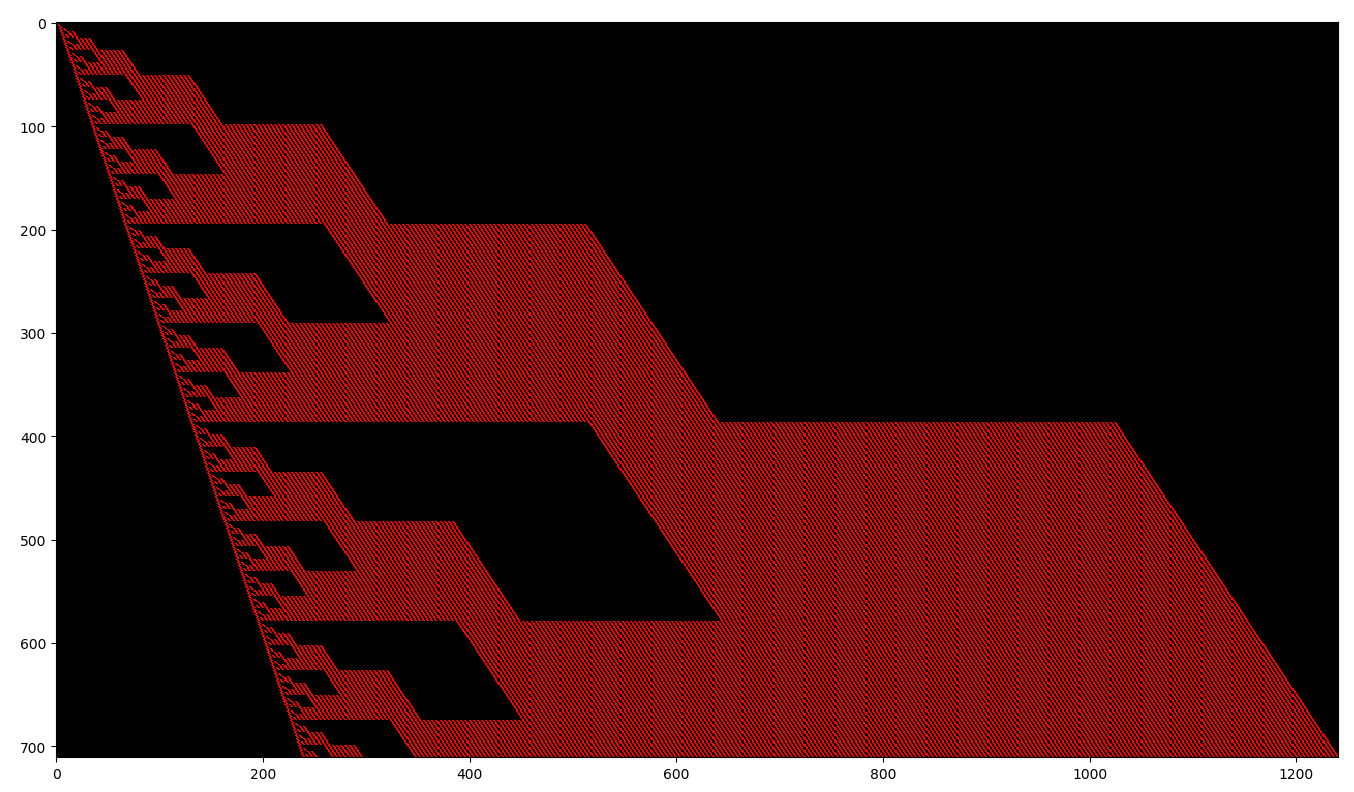
\includegraphics[width=0.8\textwidth]{19.png}
\caption{HNR \#19, tape head at left end for up to 300000 steps.}
\end{figure}

\begin{figure}[H]
\centering
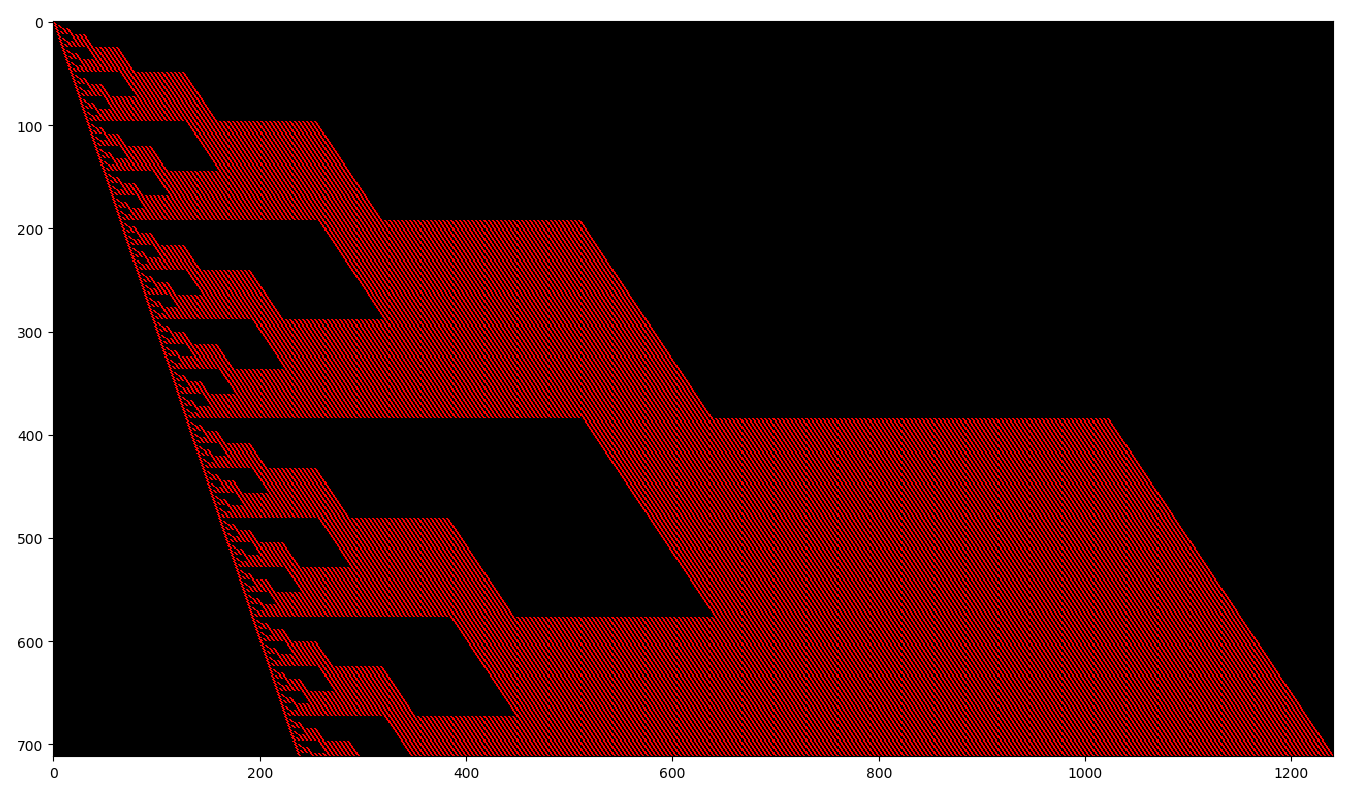
\includegraphics[width=0.8\textwidth]{42.png}
\caption{HNR \#42 similarly. These two require but a routine proof.}
\end{figure}

\clearpage
\phantomsection
\addcontentsline{toc}{section}{20}
\section*{20}
Let
\begin{align*}
T &= 1001001000\\
U &= 10010010010101001101\\
V &= 1010011010\\
W &= 10011001001001010.\\
\end{align*}
Then we observe the following:
\begin{table}[H]
\texttt{
\begin{tabular}{rrl}
22613&E& $T^{09}V^{1.5}WU^{03.5}00i$\\
70779&E& $T^{16}V^{2.5}WU^{07.5}00i$\\
145633&E&$T^{23}V^{3.5}WU^{11.5}00i$\\
247175&E&$T^{30}V^{4.5}WU^{15.5}00i$\\
375405&E&$T^{37}V^{5.5}WU^{19.5}00i$\\
530323&E&$T^{44}V^{6.5}WU^{23.5}00i,$
\end{tabular}}
\end{table}
where the half-integer indicates an additional half a repetition.

So at intervals of $48166+26688k,$ the machine just adds seven $T$s, one $V$, and four $U$s.

So the proof for HNR\#20 will be easy if possibly arduous.

\clearpage
\phantomsection
\addcontentsline{toc}{section}{22}
\section*{22}

\begin{figure}[H]
\centering
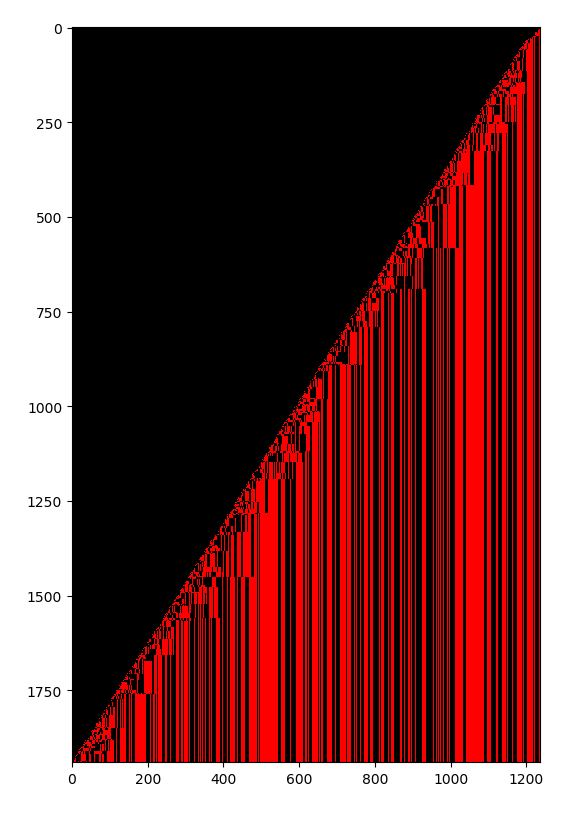
\includegraphics[width=0.8\textwidth]{22.png}
\caption{HNR \#22, tape head at left end for 199576 steps.}
\end{figure}

\begin{figure}[H]
\centering
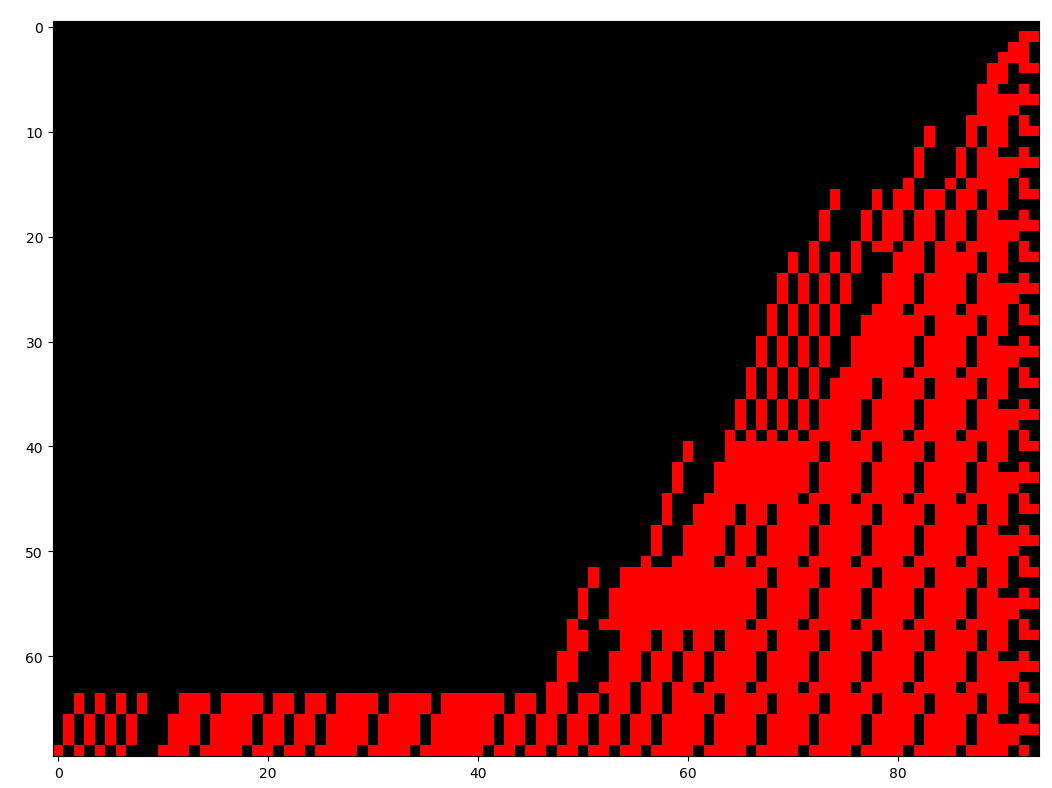
\includegraphics[width=0.8\textwidth]{22r.png}
\caption{HNR \#22, tape head at right end for 4606 steps.\\
It does not return to the right by step 3000000.}
\end{figure}

\clearpage
\phantomsection
\addcontentsline{toc}{section}{23=29}
\section*{23=29}

\begin{table}[H]
\texttt{
\begin{tabular}{rrl}
888&C&$(10)^{2}0(100)^{8}(10)^{7}i$\\
2820&C&$(10)^{2}0(100)^{18}(10)^{9}i$\\
7082&C&$(10)^{2}0(100)^{32}(10)^{11}i$\\
15114&C&$(10)^{2}0(100)^{50}(10)^{13}i$\\
28716&C&$(10)^{2}0(100)^{72}(10)^{15}i$\\
50048&C&$(10)^{2}0(100)^{98}(10)^{17}i$\\
81630&C&$(10)^{2}0(100)^{128}(10)^{19}i$\\
126342&C&$(10)^{2}0(100)^{162}(10)^{21}i$\\
187424&C&$(10)^{2}0(100)^{200}(10)^{23}i$
\end{tabular}}
\end{table}
The step differences are 1932, 4262, 8032, 13602, 21332, 31582, 44712, and 61082;\\
thus the second differences are 2330, 3770, 5570, 7730, 10250, 13130, and 16370,
the third differences are 1440, 1800, 2160, 2520, 2880, and 3240,
and the fourth differences are all 360.

So this machine will be fairly easy to prove never halts.

\clearpage
\phantomsection
\addcontentsline{toc}{section}{26}
\section*{26}

\begin{figure}[H]
\centering
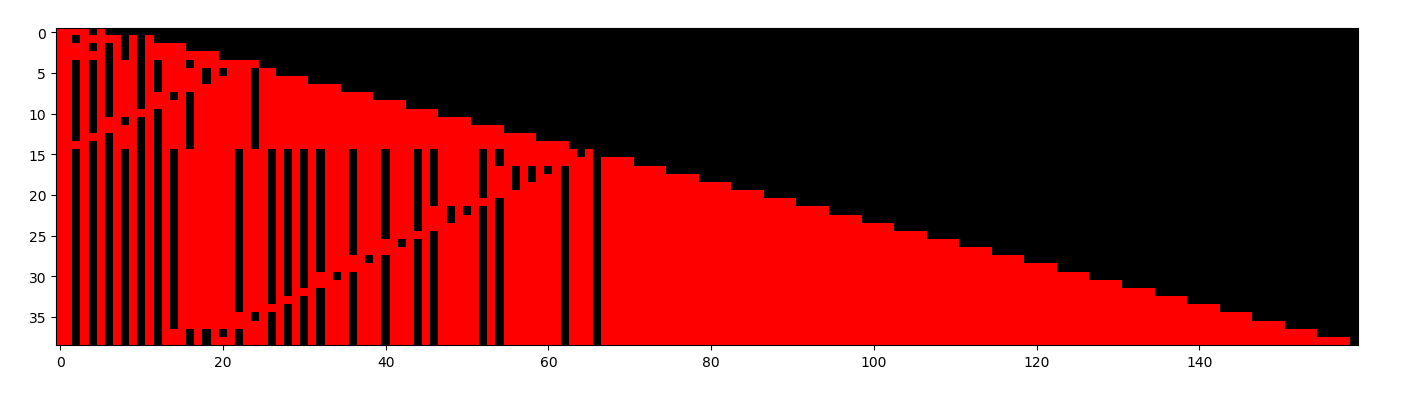
\includegraphics[width=\textwidth]{26.png}
\caption{HNR \#26, tape head at right end for 151029682 steps.\\
Each step number is roughly twice the previous.}
\end{figure}
The steps when HNR\#26 has reached the right end are 20, 84, 120, 184, 318, 343, 371, 435, 579, 859, 1431,
2583, 4879, 9483, 18695, 34848, 34858, 34902, 34966, 35102, 35382, 35954, 37110, 39406, 44006, 53218, 71650,
108506, 182234, 329682, 624594, 1214410, 2394054, 4753346, 9471934, 18909118, 37783478, 75532222, 151029686
shown in this picture. Denote this sequence by $a,$ and let $\Delta s$ denote the sequence $s_{i+1}-s_i$
for any sequence $s.$ Then it is observed that $\Delta a - \Delta^2 a$ is the sequence
92, 8, -6, 243, 22, -8, -16, 8, -12, -8, 8, -12, -4, 2271, 32296, -24, 24, -8, -8, -12, -12, 16, -8, -12,
-8, 8, -16, 8, -16, 8, -12, -4, -4, -8, 8, -24, 24.

In other words, the intervals between steps fail to double by very little in most transitions,
and where they fail greatly coordinates with the transition around the 15 mark in the picture.

\clearpage
\phantomsection
\addcontentsline{toc}{section}{BL\_2}
\section*{BL\_2}

\begin{table}[H]
\texttt{
\hspace*{-0.75in}
\begin{tabular}{rrl}
10&C&$i1011$\\
51&C&$i101(110)^{2}11$\\
214&C&$i101(110)^{1}1(110)^{5}11$\\
1063&C&$i101(110)^{1}1(110)^{2}10(110)^{12}11$\\
5834&C&$i101(110)^{1}1(110)^{2}10(110)^{2}1(110)^{32}11$\\
34397&C&$i101(110)^{1}1(110)^{2}10(110)^{2}1(110)^{6}1(110)^{80}11$\\
209800&C&$i101(110)^{1}1(110)^{2}10(110)^{2}1(110)^{6}1(110)^{14}1(110)^{200}11$\\
1298303&C&$i101(110)^{1}1(110)^{2}10(110)^{2}1(110)^{6}1(110)^{14}1(110)^{34}1(110)^{500}11$\\
8082056&C&$i101(110)^{1}1(110)^{2}10(110)^{2}1(110)^{6}1(110)^{14}1(110)^{34}1(110)^{84}1(110)^{1250}11$\\
50432059&C&$i101(110)^{1}1(110)^{2}10(110)^{2}1(110)^{6}1(110)^{14}1(110)^{34}1(110)^{84}1(110)^{209}1(110)^{3125}11$\\
315021908&C&$i101(110)^{1}1(110)^{2}10(110)^{2}1(110)^{6}1(110)^{14}1(110)^{34}1(110)^{84}1(110)^{209}1(110)^{522}10(110)^{7812}11$\\
\end{tabular}}
\end{table}
Let $a_i$ and $b_i$ denote the exponents of the last and second to last swath of 110s during a given step
when the tape head has reached the left edge of the tape anew, as written above.

Then it appears to be the case that
\begin{align*}
b_{i+1}&=\lceil a_i/6\rceil+t\\
a_{i+1}&=\lfloor5a_i/2\rfloor
\end{align*}
where $t$ is 1 if $a_i$ is $5\pmod6$ and 0 otherwise.

Seems the step number tends to multiplying by $25/4$ from each step to the next.

The sequence of differences in step number seems to tend to multiplying by $25/4$ as well,
with the error incurred by assuming this being about
$11\%, 4.4\%, 1.8\%, .71\%,$ and $.23\%$ of the previous difference by the end.
Also, the ratio between each of these errors and the next seems to be very close to $5/2$ half the time.

Thus denote by $\{x_i\}_{i=0}^{10}$ the sequence of step numbers mentioned above, and let
\begin{align*}
y_i&=x_{i+1}-x_{i},\\
z_i&=\frac{25}{4}y_i-y_{i+1},\textrm{ and}\\
w_i&=\frac{5}{2}z_i-z_{i+1}.\\
\end{align*}
Let us align the values we get for $\{w_i\}_{i=0}^{7}$ against $a_i\pmod6$:
\begin{table}[H]
\begin{tabular}{llllllllll}
63.375&-110.875&82.375&23.625&23.625&23.625&23.625&23463.375&{}&{}\\
0&2&5&0&2&2&2&2&2&5
\end{tabular}
\caption*{So it seems that $w_i$ is $23\sfrac{5}{8}$ whenever all of $a_i,a_{i+1},$ and $a_{i+2}$ are not $5\pmod6.$}
\end{table}
Although it is too early to tell, it seems likely that HNR\#BL\_2 will not be very difficult.

\clearpage
\phantomsection
\addcontentsline{toc}{section}{30=41}
\section*{30=41}

\begin{figure}[H]
\centering
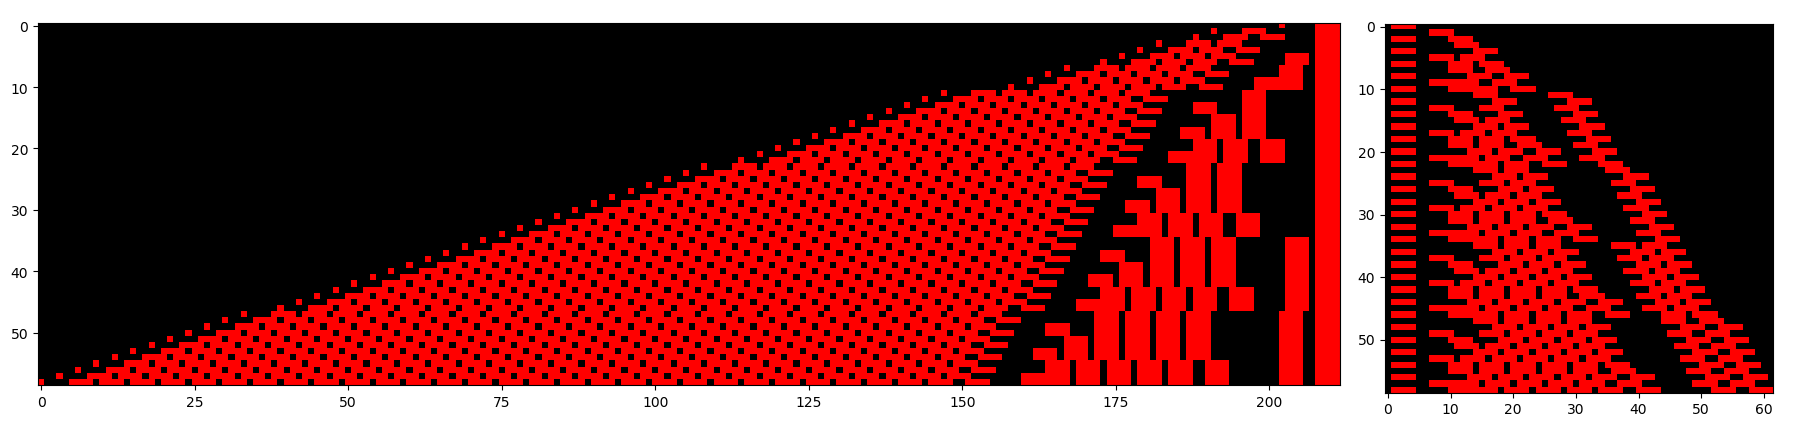
\includegraphics[width=\textwidth]{30.png}
\caption{HNR \#30, tape head at left end for 30000 steps.\\
The second image shows it left-justified with the beginning repetitive portion deleted.}
\end{figure}

\begin{figure}[H]
\centering
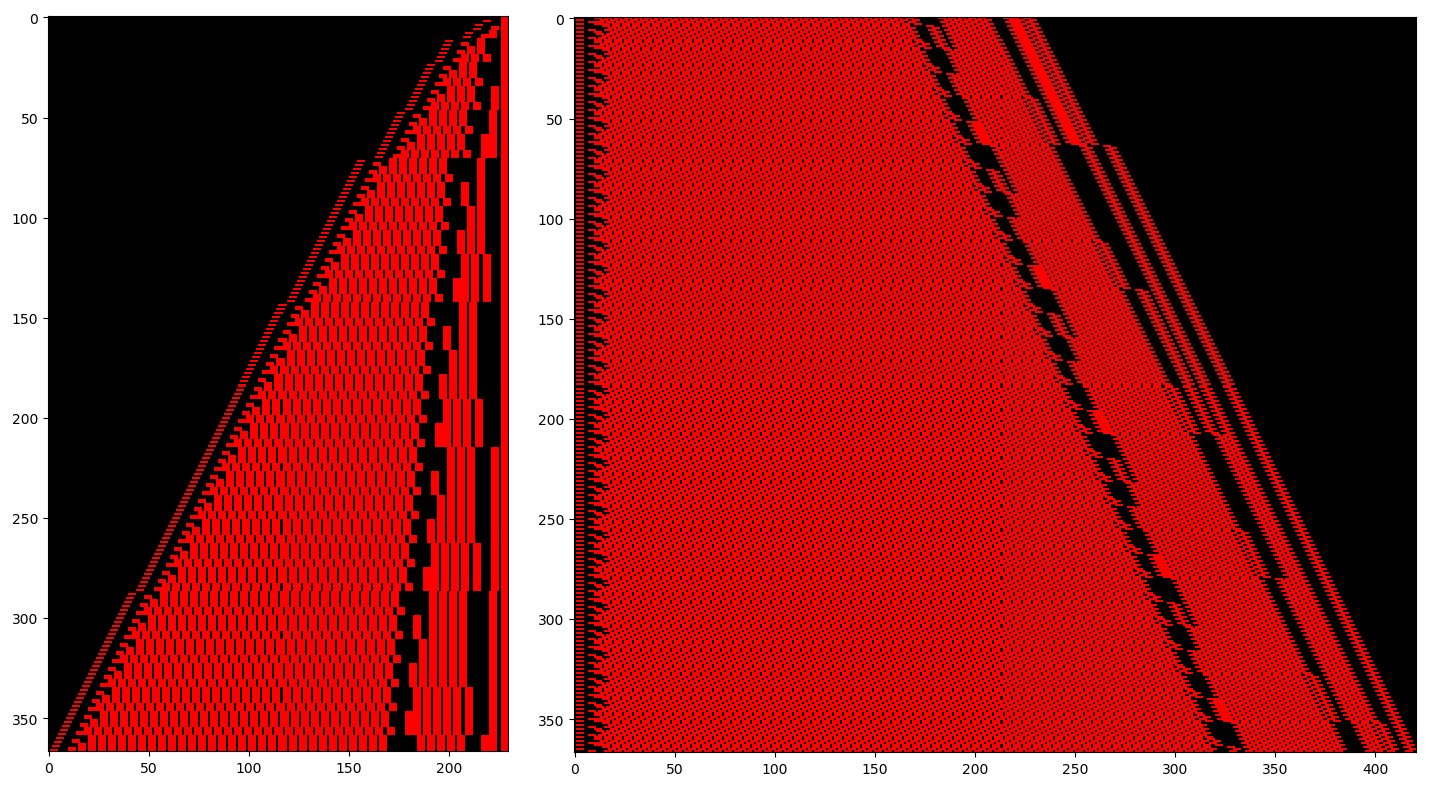
\includegraphics[width=\textwidth]{30long.png}
\caption{Tape head at left, repetitive portion deleted, right-justified, 1000000 steps.\\
The second image shows the same left-justified from step 1000000 to 3939415.}
\end{figure}

The action of this machine appears to be of a fractal nature, but it is more difficult to describe
than that of HNR\#16 or 19.

On the next page, we will see that looking at moments when the tape head is on the right side
helps us figure out much more easily what to do to prove that this machine never halts.

\newpage

Looking at moments when the tape head is on the right gives us a much clearer picture of what to do.
If we list all steps from 31 to 300000000 when the tape head is on the right, it follows a 5/2/5/5/5
pattern where the 5 is E-B-C-D-A and the 2 is C-D. Taking only those C moments from the 2,
hence, rows $5\pmod{22}$ indexing from 0, we obtain the following steps:

\begin{table}[H]
\texttt{
\begin{tabular}{rrr}
92&C&$(11110)^{2}11i$\\
1842&C&$(11110)^{6}1^{14}(11110)^{2}11i$\\
42652&C&$(11110)^{36}1^{14}(11110)^{6}1^{14}(11110)^{2}11i$\\
1376222&C&$(11110)^{216}1^{14}(11110)^{36}1^{14}(11110)^{6}1^{14}(11110)^{2}11i$\\
48568752&C&$(11110)^{1296}1^{14}(11110)^{216}1^{14}(11110)^{36}1^{14}(11110)^{6}1^{14}(11110)^{2}11i$\\
\end{tabular}}
\end{table}
Studying the step numbers, it appears that their ratio is trending towards 36, which is not surprising
given the lengths of strings involved. Thus let the sequence of five steps above be $\{x_i\}_{i=0}^4,$
and define $y_i=36x_i-x_{i+1}.$ We obtain
$$1470, 23660, 159250, 975240.$$
The descending tens places suggest taking the difference, so let $z=\Delta y.$ We get
$$22190, 135590, 815990.$$
The ratios of subsequent terms are very close to 6, so let $w_i=z_{i+1}-6z_i.$

We find that $w$ is the constant sequence $2450$ of length 2 so far.
Substituting in terms of the original sequence, this is to say
\begin{align}
2450&=-x_{i+3}+43x_{i+2}-258x_{i+1}+216x_i,\textrm{ or}\\
x_{i+3}&=43x_{i+2}-258x_{i+1}+216x_i-2450.\label{recx}
\end{align}
Since $43\cdot48568752-258\cdot1376222+216\cdot42652-2450=1742601442,$
let us inspect step 1742601442 to confirm that our result was not just an artifact of having
too many parameters available to adjust. The output of the Java program Turing,
when written with exponents using blit30end.py, gives:
$$1742601442~\texttt{C}~(11110)^{7776}1^{14}(11110)^{1296}1^{14}(11110)^{216}1^{14}(11110)^{36}1^{14}(11110)^{6}1^{14}(11110)^{2}11i$$
Thus the following is overwhelmingly likely to be true:
\begin{conjecture}
At steps $\{x_i\}_{i=1}^{\infty}$ where $x_1=92,~x_2=1842,$ and $x_3=42652,$ and \eqref{recx},
HNR\#30 is in state C with tape head at its rightmost 1 bit and tape
$$\left(\prod_{j=1}^i (11110)^{6^{i+1-j}}1^{14}\right)(11110)^2 111.$$
\end{conjecture}
The proof will likely be not too difficult, but it might be very arduous.

\clearpage
\phantomsection
\addcontentsline{toc}{section}{33}
\section*{33}

\begin{figure}[H]
\centering
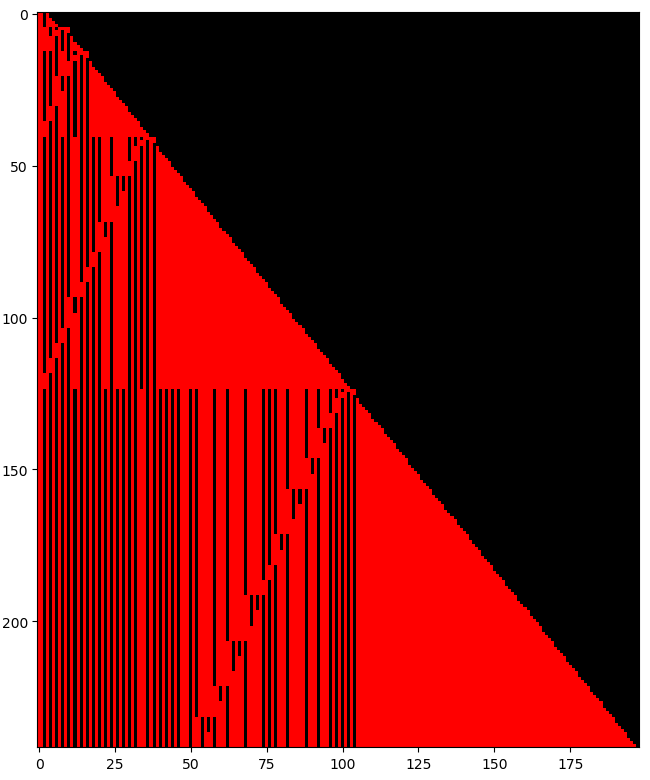
\includegraphics[width=\textwidth]{33.png}
\caption{Tape head at right from step 10 to step 238493660.\\
There is not another moment in the first 300 million steps.}
\end{figure}
It almost always hits the right in A and stays on the right for five steps in A-D-B-E-A,
except for moments during the four clear transitional periods shown where it does E and then D-A eight steps later;
these are at steps 74, 177, 1980 and 3612743.

If we instead try to determine moments when it has reached the left, we get an extraordinary sparse set of steps:
\begin{table}[H]
\texttt{
\begin{tabular}{rcl}
47&E&$1^6I$\\
144&E&$1^{12}I$\\
1785&E&$1^{18}IOIII$\\
3612042&E&$1^{20}IIOOIOIIIIOIIIII$
\end{tabular}}
\caption*{Tape head at leftmost 1. $I=0001,O=0000.$}
\end{table}
The 47, 144, 1785 and 3612042 correspond to a mere 27, 33, 205 steps and 701 steps, respectively, behind the
four clear transitional periods shown in the figure where it was on the left.
So it is safe to assume that it never gets back to the left until it's done ``doing its computation''
on the previous string, whatever that may mean to it.

\begin{table}[H]
\texttt{
\begin{tabular}{rcl}
74&E&1111010111i\\
177&E&1101010111010111i\\
1980&E&1$(10)^{5}11(10)^{4}11101111101010111i$\\
3612743&E&$1(10)^{16}11(10)^{6}111010111110111011111011111010101110111110111011101010111i$
\end{tabular}}
\caption*{Tape head at rightmost bit for transitional period.}
\end{table}

It does not reach the left again within the first 3 billion steps.

Probably a significant acceleration would be required to find even the next moment when it reaches the left.
It also might be a good idea to run experiments like $1^{6n}0001~E$ with the tape head on the left
and take a look at what the tape looks like the first moment the head hits the right.

Maybe it's doing something like Ackermann's function.

\clearpage
\phantomsection
\addcontentsline{toc}{section}{34}
\section*{34}

\begin{figure}[H]
\centering
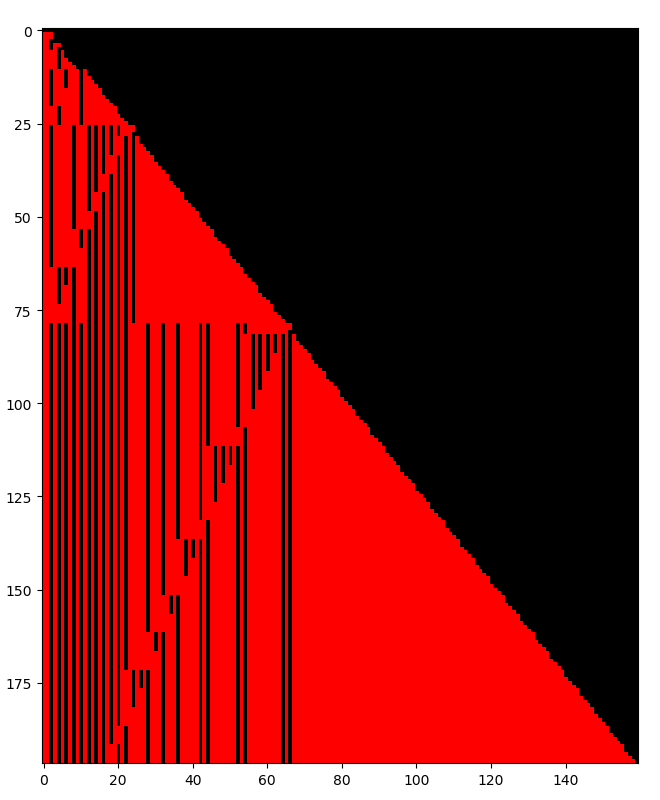
\includegraphics[width=0.5\textwidth]{34.png}
\caption{Tape head at right until step 218136190.\\
There is not another moment in the first 300 million steps.}
\end{figure}

This machine seems to be very similar to machine \#33;
it even seems to have the same orientation and with Skelet's program's choice use the same states
A-D-B-E-A for usual rightmost bit moments and E-D-A for transitional moments,
only with two instead of eight steps from the E to the D.

\begin{table}[H]
\texttt{
\begin{tabular}{rcl}
12&D&$i011$\\
51&D&$i01^{3}0I$\\
90&D&$i01^{4}I1$\\
391&D&$i01^{9}0OII$\\
32112&D&$i01^{24}IIIIIOIOOI$
\end{tabular}}
\caption*{Tape head at leftmost 1. $I=0001,O=0000.$\\
There are no other steps under 3 billion (other than adjacent steps) where the tape head is on the left.}
\end{table}



\clearpage
\phantomsection
\addcontentsline{toc}{section}{35}
\section*{35}

\begin{figure}[H]
\centering
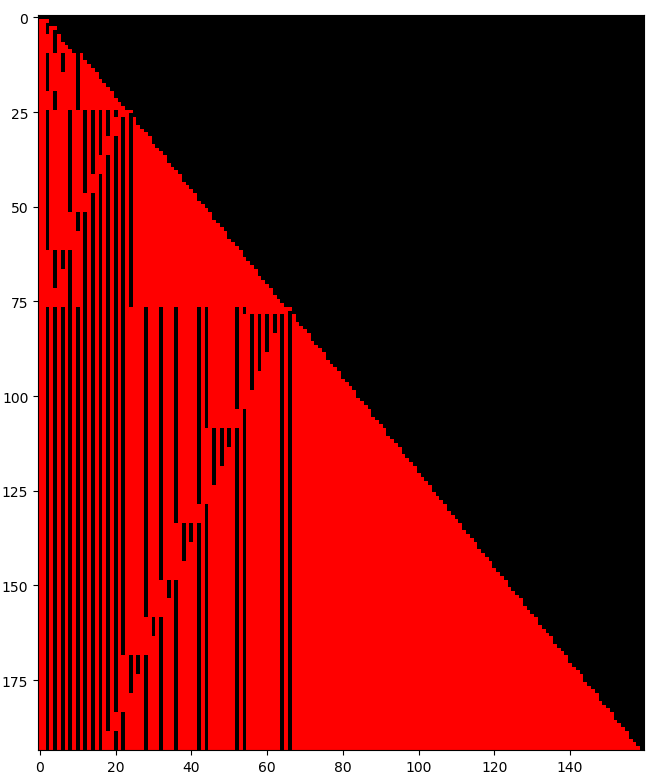
\includegraphics[width=0.5\textwidth]{35.png}
\caption{Tape head at right until step 201356448.\\
There is not another moment in the first 300 million steps.}
\end{figure}

This machine seems to be very similar to machine \#s 33 and 34;
it even seems to have the same orientation and with Skelet's program's choice use the same states
A-D-B-E-A for usual rightmost bit moments. It uses E-A, adjacent steps, for transitional moments.

\begin{table}[H]
\texttt{
\begin{tabular}{rcl}
10&D&$i011$\\
45&D&$i01^{3}0I$\\
80&D&$i01^{4}I1$\\
355&D&$i01^{9}0OII$\\
29630&D&$i01^{24}IIIIIOIOOI$
\end{tabular}}
\caption*{Tape head at leftmost 1. $I=0001,O=0000.$\\
There are no other steps under 3 billion (other than adjacent steps) where the tape head is on the left.}
\end{table}
Notice that these configurations are the exact same, even with the same orientation and state, as those of HNR\#34.
The differences in step number between a leftmost configuration of HNR\#34 and the equivalent configuration of \#35
are 2, 6, 10, 36, 2482.

%\clearpage
\phantomsection
\addcontentsline{toc}{section}{36}
\section*{36}

\begin{figure}[H]
\centering
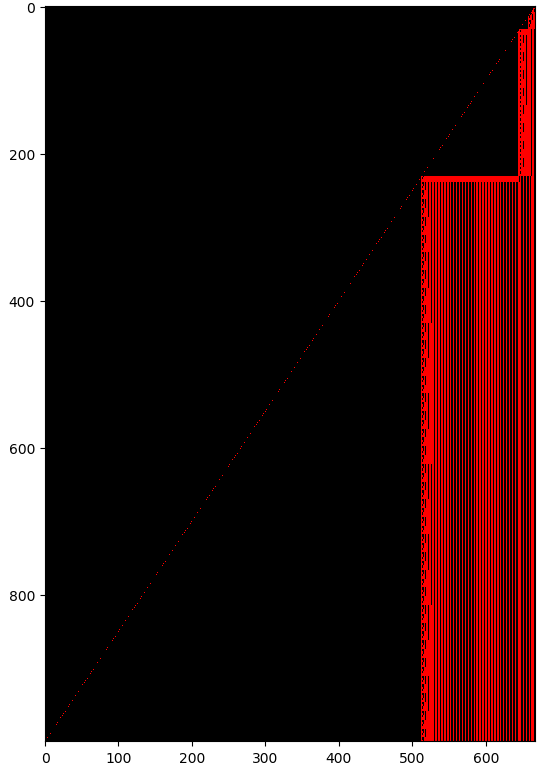
\includegraphics[width=\textwidth]{36.png}
\end{figure}

The figure above shows the steps where the tape head is at left until step 144081.
It never seems to make it to the right after step 40.

\begin{figure}[H]
\centering
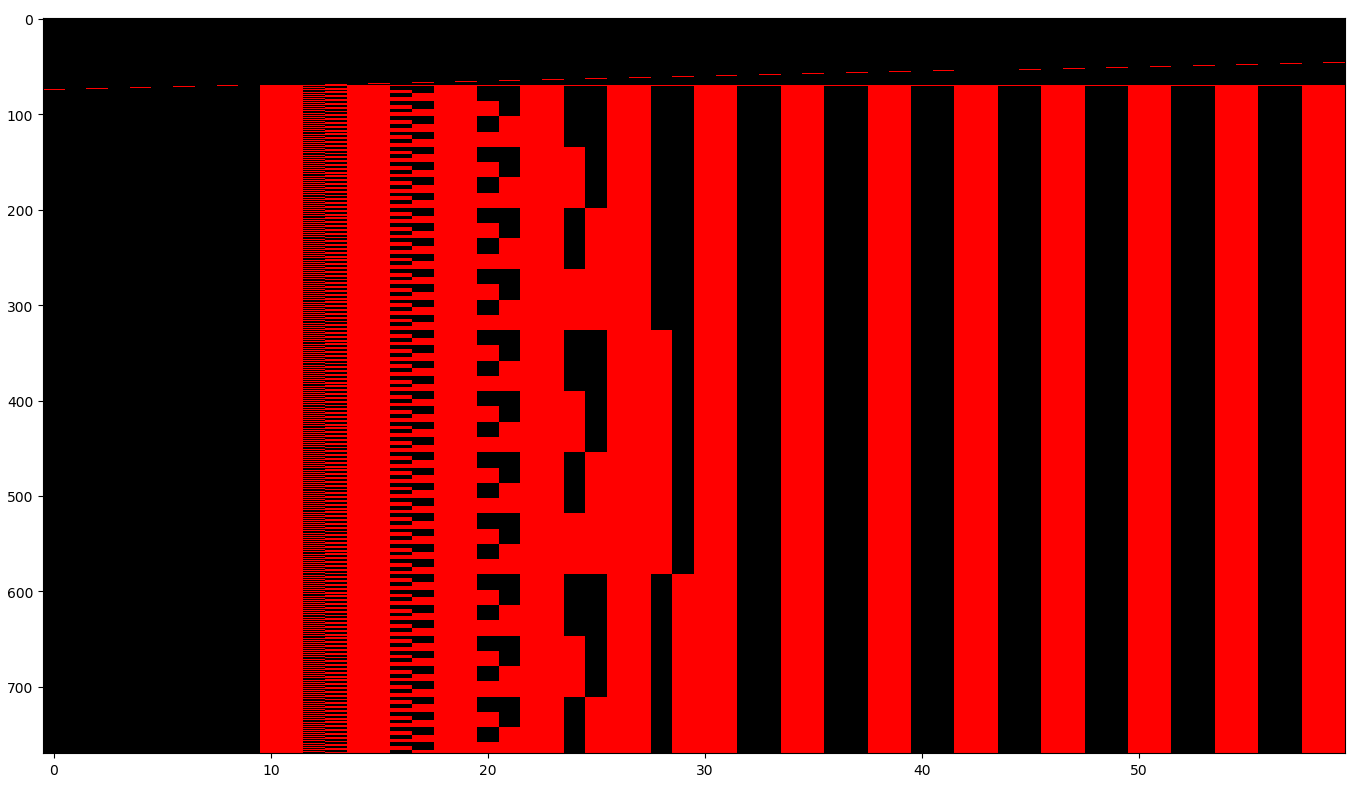
\includegraphics[width=\textwidth]{36-2.png}
\caption{Zooming in on a particular part of the image and stretching the aspect ratio
reveals that it is definitely binary counting going on.}
\end{figure}

\newpage

\begin{table}[H]
\texttt{
\begin{tabular}{rcr}
29&D&o00011111\\
64&D&o011011101101\\
100&D&o0000011001111101\\
120&D&o000000011101111101\\
146&D&o00000000011011111101\\
174&D&o0000000000011111111101\\
265&D&o0110111111111110110011011\\
277&D&o000111111111111110110011011\\
\end{tabular}}
\caption*{Tape head at left from 29 to 265. Recall that at step 40 it is on the right.\\
If there were an even number of intervening 0s, the machine would halt.}
\end{table}

Any journey ``there and back again'' from a configuration as above, in state D on the left at a 0
with an odd number of intervening 0s before a string beginning with 1, consists of the following phases:

\begin{enumerate}
\item B-D alternation going to the right. By parity this necessarily culminates in a configuration like
\texttt{186 D 111111111111i1111111101}.
\item A-E alternation going to the right (after one left step). This will yield a step like
\texttt{160 E 111111111101o11111101} or \texttt{197 A 111111111111010101010o1}.
\item C-D-A-C going to the left in the latter case; the same beginning with the D in the former case.
How this ends could in theory depend on how many 1s there were $\pmod4$. This phase 
in the first string of 1s after the first string of 0s at the starting step, such as 174, where there were 9.
\item Once it has gotten left of the ``tie'' bit (as in step 186),
the latter case goes into an A-E-A-C-D phase,
moving 1 to the left every 5 steps, followed by one final A-C-D at extreme left.
The former case goes into straight Cs, going left.
\end{enumerate}
This accounts for the vastly different results of ending at step 174 and 265 on the left.
In fact, it seems to be the case that we get this ``transition-producing'' behavior
only when the number of 1s in that swath is $1\pmod4.$
In all cases, the whole string should probably be interpreted as a usual binary number,
with least significant digit on the left, but with an extra pair of 1s between each pair of digits.
One can see how the machine is thus counting up:

\begin{table}[H]
\texttt{
\begin{tabular}{rcr}
5717&D&$o0^{099}111111111101111110011011$\\
5941&D&$o0^{101}110011001111111110011011$\\
6153&D&$o0^{103}111011001111111110011011$\\
6371&D&$o0^{105}110111001111111110011011$\\
6591&D&$o0^{107}111111001111111110011011$\\
6823&D&$o0^{109}110011101111111110011011$\\
7051&D&$o0^{111}111011101111111110011011$\\
7285&D&$o0^{113}110111101111111110011011$\\
7521&D&$o0^{115}111111101111111110011011$\\
7771&D&$o0^{117}110011011111111110011011$\\
8015&D&$o0^{119}111011011111111110011011$\\
8265&D&$o0^{121}110111011111111110011011$\\
8517&D&$o0^{123}111111011111111110011011$\\
8781&D&$o0^{125}110011111111111110011011$\\
9041&D&$o0^{127}111011111111111110011011$\\
9307&D&$o0^{129}110111111111111110011011$\\
9575&D     &$o0^{131}1111111111111111{\textcolor{red}{10}}011011$\\
10414&D&$o0^{3}1^{134}01{\textcolor{red}{10}}0110011001101011011$\\
10694&D&$o0^{5}(1100)^{33}1111100110011001101011011$\\
\end{tabular}}
\caption*{Since there are 17 1s in a row in the second-to-last row, the machine is no longer able to interpret
everything it meets in the ``binary number in pairs with pairs of 1s ahead of each pair of bits'' format.}
\end{table}
So the machine has set up a whole new task for itself on step 10414, so to speak;
or, it has set up the same old task for itself with a whole new number.
It \emph{is} able to view this new format as a binary number through the 136th tape bit (68th number bit),
but the 138th violates the format, and so after $2^{66}$ passes after step 10694
it will increment this old new problem bit-pair and create a whole new number for itself,
$2*2^{66}+5+1$ tape bits longer than the old number, reinterpreting this as a binary number of
$2^{66}+3$ numerical bits to count all the way up. 
It will continue turning the counting number (of 0s) it has created for itself linearly with each pass
into a space into which to count up in binary, extending by pairs of 0s to the left all the while (see also Figure).
The problem bits (shown in red) recede to the left at each of these transitions.

If this analysis is correct\textemdash and it clearly needs to be made more precise\textemdash then HNR\#36 never halts.

\newpage

We make it more precise here.
\begin{lemmastar}
Let HNR\#36 be in state $D$ with tape $o0^{m}1^{n}0x,$
where $m$ is odd, $n$ is positive, and $x$ is any string.
Then it will return to another configuration with the same property later.
\end{lemmastar}
\begin{figure}[H]
\centering
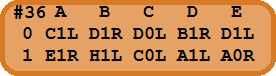
\includegraphics[width=0.5\textwidth]{HNR36.png}
\end{figure}
\begin{proof}
Refer to the phases mentioned above.
\begin{table}[H]
\begin{tabular}{rllll}
        &0    &D&$o0^{m}1^{n}0$\\
$\vdash$&m+1  &D&$1^{m+1}i1^{n-1}0$\\
$\vdash$&m+3  &E&$1^{m+1}i1^{n-1}0$\\
$\vdash$&m+n+3&E&$1^{m+1}(01)^{n/2}o$,     &$n$ even, or\\
        &m+n+3&A&$1^{m+1}(01)^{(n-1)/2}0o$,&$n$ odd.
\end{tabular}
\end{table}

If $n$ is even, one obtains
\begin{table}[H]
\begin{tabular}{rllll}
        &m+2n+4 &D&$1^{m}i(0011)^{n/4}1$\\
$\vdash$&6m+2n+5&A&$o1^{m+2}011(0011)^{\frac{n}{4}-1}1$\\
$\vdash$&6m+2n+7&D&$o01^{m+3}011(0011)^{\frac{n}{4}-1}1$, &$n\equiv0\pmod4$, or\\
        &m+2n+4 &C&$1^{m}i11(0011)^{(n-2)/4}1$\\
$\vdash$&2m+2n+5&C&$o0^{m+1}11(0011)^{(n-2)/4}1$\\
$\vdash$&2m+2n+6&D&$o0^{m+2}11(0011)^{(n-2)/4}1$,&$n\equiv2\pmod4$.
\end{tabular}
\end{table}
The $n\equiv0\pmod4$ case is from the A-E-A-C-D phase mentioned above.
So in the first case, we end up with one 0 after the $D,$
whereas in the second case, we end up with $m+2$ 0s after the $D.$

If $n$ is odd, one obtains
\begin{table}[H]
\begin{tabular}{rllll}
        &m+n+5 &D&$1^{m+1}(01)^{(n-1)/2}<01$\\
$\vdash$&m+2n+6&D&$1^{m}i(0011)^{(n-1)/4}01$,&$n\equiv1\pmod4,$ or\\
        &m+2n+6&C&$1^{m}i11(0011)^{(n-3)/4}01$,&$n\equiv3\pmod4.$
\end{tabular}
\end{table}
by A-C-C-D. Thus the $1\pmod4$ case finishes out like the $0\pmod4$ case,
and the $3\pmod4$ case finishes out like the $2\pmod4$ case.
\end{proof}
Thus HNR\#36 never halts.

\clearpage
\phantomsection
\addcontentsline{toc}{section}{37}
\section*{37}

\begin{table}[H]
\texttt{
\begin{tabular}{rcr}
12&A&$(10)^{3}$\\
71&A&$(10)^{3}1(10)^{3}$\\
400&A&$(10)^{9}1(10)^{3}1(10)^{3}$\\
2835&A&$(10)^{27}1(10)^{9}1(10)^{3}1(10)^{3}$\\
23252&A&$(10)^{81}1(10)^{27}1(10)^{9}1(10)^{3}1(10)^{3}$\\
202591&A&$(10)^{243}1(10)^{81}1(10)^{27}1(10)^{9}1(10)^{3}1(10)^{3}$\\
1803480&A&$(10)^{729}1(10)^{243}1(10)^{81}1(10)^{27}1(10)^{9}1(10)^{3}1(10)^{3}$\\
16172075&A&$(10)^{2187}1(10)^{729}1(10)^{243}1(10)^{81}1(10)^{27}1(10)^{9}1(10)^{3}1(10)^{3}$\\
145371292&A&$(10)^{6561}1(10)^{2187}1(10)^{729}1(10)^{243}1(10)^{81}1(10)^{27}1(10)^{9}1(10)^{3}1(10)^{3}$\\
\end{tabular}}
\caption*{Moments when the tape head is on the right.}
\end{table}
HNR\#37 will thus clearly be a simple one to prove never halts.

\clearpage
\phantomsection
\addcontentsline{toc}{section}{40}
\section*{40}

\begin{figure}[H]
\centering
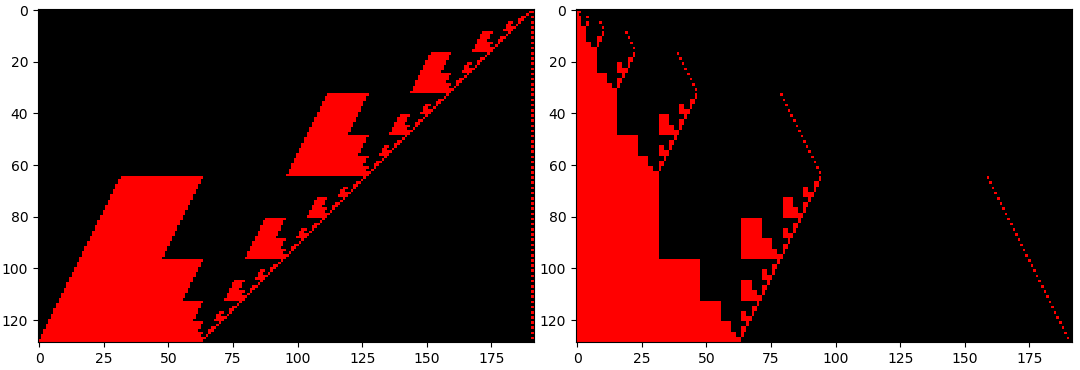
\includegraphics[width=\textwidth]{40.png}
\caption{Tape head on the right, right-justified and left-justified respectively.}
\end{figure}

\begin{figure}[H]
\centering
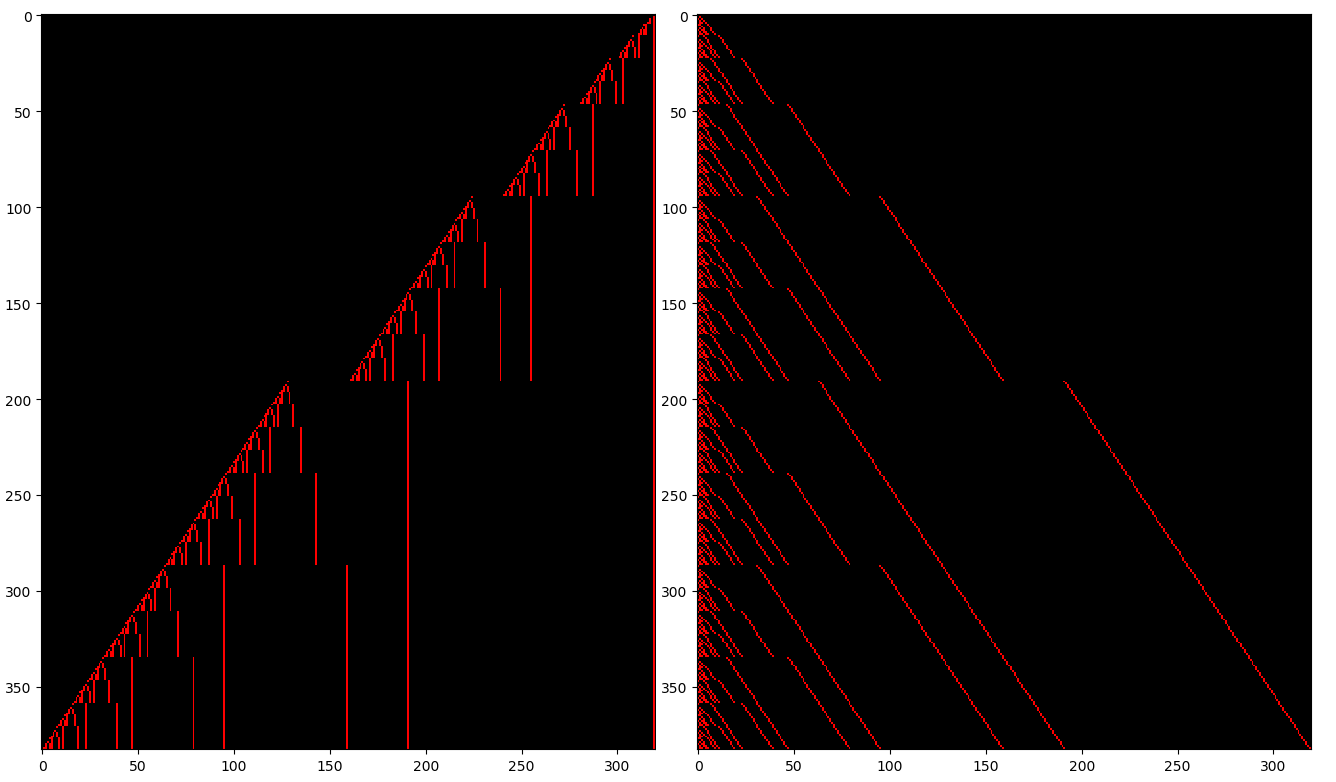
\includegraphics[width=\textwidth]{40l.png}
\caption{Tape head on the left, right-justified and left-justified respectively.}
\end{figure}
HNR\#40 seems to just want to draw a fractal, so I'm lumping it in with the ``easy but arduous to prove.''

\clearpage
\phantomsection
\addcontentsline{toc}{section}{43}
\section*{43}

\begin{table}[H]
\texttt{
\begin{tabular}{rcr}
87&C&$o001101111111$\\
219&C&$o001101(1110110)^{1}1111111$\\
569&C&$o00110111111(1110110)^{2}1111111$\\
1536&C&$o001101^{11}(1110110)^{4}1111111$\\
4472&C&$o001101(1110110)^{1}1^{11}(1110110)^{8}1111111$\\
14462&C&$o00110111111(1110110)^{2}1^{11}(1110110)^{16}1111111$\\
50837&C&$o001101^{11}(1110110)^{4}1^{11}(1110110)^{32}1111111$\\
189101&C&$o001101(1110110)^{1}1^{11}(1110110)^{8}1^{11}(1110110)^{64}1111111$\\
727795&C&$o00110111111(1110110)^{2}1^{11}(1110110)^{16}1^{11}(1110110)^{128}1111111$\\
2853770&C&$o001101^{11}(1110110)^{4}1^{11}(1110110)^{32}1^{11}(1110110)^{256}1111111$\\
\end{tabular}}
\caption*{Moments when the tape head is on the left.}
\end{table}
Non-halting of HNR\#43 will thus clearly be an easy but possibly arduous proof.

\end{document}